\documentclass[aspectratio=169, 10pt]{beamer}
\usepackage{fontspec}
\usefonttheme{professionalfonts}
\setmainfont{Times New Roman}
\setsansfont{Times New Roman}

\usepackage{amsmath, amssymb}
\usepackage{booktabs, colortbl, multirow}
\usepackage{tikz}
\usetikzlibrary{shapes, arrows.meta, positioning, calc, matrix, fit, backgrounds, decorations.pathreplacing}
\usepackage{graphicx}
\graphicspath{{figures/}{figures/pdf_assets/}{figures/pdf_assets_08/}}

\usetheme{Madrid}
\usecolortheme{whale}
\setbeamertemplate{navigation symbols}{}

% Custom Professional Color Palette
\definecolor{mainnavy}{RGB}{26, 54, 93}
\definecolor{accentteal}{RGB}{13, 92, 117}
\definecolor{teal}{RGB}{13, 92, 117}
\definecolor{warmorange}{RGB}{217, 119, 6}
\definecolor{crimsonred}{RGB}{220, 38, 38}
\definecolor{emeraldgreen}{RGB}{5, 150, 105}
\definecolor{slate}{RGB}{51, 65, 85}
\definecolor{lightbg}{RGB}{248, 250, 252}
\definecolor{boxblue}{RGB}{239, 246, 255}
\definecolor{boxgreen}{RGB}{240, 253, 244}
\definecolor{boxorange}{RGB}{255, 251, 235}
\definecolor{boxred}{RGB}{254, 242, 242}

\setbeamercolor{structure}{fg=mainnavy}
\setbeamercolor{title}{bg=mainnavy, fg=white}
\setbeamercolor{frametitle}{bg=mainnavy, fg=white}
\setbeamercolor{block title}{bg=mainnavy, fg=white}
\setbeamercolor{block body}{bg=lightbg, fg=slate}
\setbeamercolor{block title example}{bg=accentteal, fg=white}
\setbeamercolor{block body example}{bg=lightbg, fg=slate}
\setbeamercolor{block title alerted}{bg=crimsonred, fg=white}
\setbeamercolor{block body alerted}{bg=boxred, fg=slate}

% Custom Footline ensuring exact x / 46 numbering
\setbeamertemplate{footline}{%
  \leavevmode%
  \hbox{%
  \begin{beamercolorbox}[wd=.333333\paperwidth,ht=2.5ex,dp=1.1ex,center]{author in head/foot}%
    \usebeamerfont{author in head/foot}Chuyên đề Thị giác Máy tính
  \end{beamercolorbox}%
  \begin{beamercolorbox}[wd=.333333\paperwidth,ht=2.5ex,dp=1.1ex,center]{title in head/foot}%
    \usebeamerfont{title in head/foot}Mạng Nơ-ron Tích chập (CNN)
  \end{beamercolorbox}%
  \begin{beamercolorbox}[wd=.333333\paperwidth,ht=2.5ex,dp=1.1ex,right]{date in head/foot}%
    \usebeamerfont{date in head/foot}\insertframenumber{} / 52\hspace*{2.5ex}
  \end{beamercolorbox}}%
  \vskip0pt%
}

% Standardized Arrow & TikZ Styles
\tikzset{
  >=Stealth,
  flowarrow/.style={-{Stealth[length=2.2mm, width=1.5mm]}, thick, mainnavy},
  flowarrow_teal/.style={-{Stealth[length=2.2mm, width=1.5mm]}, thick, accentteal},
  flowarrow_red/.style={-{Stealth[length=2.2mm, width=1.5mm]}, thick, crimsonred},
  flowarrow_green/.style={-{Stealth[length=2.2mm, width=1.5mm]}, thick, emeraldgreen},
  flowarrow_orange/.style={-{Stealth[length=2.2mm, width=1.5mm]}, thick, warmorange},
  axisarrow/.style={-{Stealth[length=2.2mm, width=1.5mm]}, thick, mainnavy}
}

% Matrix styles for numerical walkthrough
\tikzset{
  cell/.style={rectangle, draw=gray!40, minimum size=0.50cm, text centered, font=\scriptsize},
  activecell/.style={rectangle, draw=mainnavy, fill=blue!15, minimum size=0.50cm, text centered, font=\scriptsize\bfseries},
  kernelcell/.style={rectangle, draw=warmorange!90!black, fill=warmorange!20, minimum size=0.50cm, text centered, font=\scriptsize\bfseries},
  outcell/.style={rectangle, draw=accentteal!90!black, fill=accentteal!20, minimum width=0.68cm, minimum height=0.68cm, text width=0.60cm, align=center, inner sep=0pt, font=\scriptsize\bfseries},
  origcell/.style={rectangle, draw=mainnavy!70!black, fill=blue!15, minimum size=0.46cm, text centered, font=\scriptsize\bfseries},
  padzero/.style={rectangle, draw=gray!35, fill=gray!10, minimum size=0.46cm, text centered, font=\scriptsize, text=gray!70!black}
}

\title[Chuyên đề CNN]{MẠNG NƠ-RON TÍCH CHẬP (CNN)}
\subtitle{Từ Nền tảng Toán học, Tiến hóa Kiến trúc đến Thực nghiệm Đối sánh \& Triển khai}
\author{}
\institute{}
\date{}

\begin{document}

% =============================================================
% SLIDE 1: TRANG TIÊU ĐỀ
\begin{document}
% =============================================================
\begin{frame}[plain]
\titlepage
\end{frame}

% =============================================================
% SLIDE 2: MỤC LỤC
% =============================================================
\begin{frame}{Mục Lục}
\centering
\vspace{0.4cm}

\begin{tikzpicture}
    % Block 1: Nền tảng kiến trúc CNN
    \node[draw=mainnavy!50, fill=mainnavy!4, rounded corners=8pt, line width=1.2pt,
          minimum width=13.0cm, minimum height=2.1cm, inner sep=10pt] (c1) at (0, 1.3) {
        \begin{minipage}{12.4cm}
            \centering
            {\fontsize{20}{26}\selectfont\bfseries\color{mainnavy} Nền tảng kiến trúc CNN}
        \end{minipage}
    };
    \draw[fill=mainnavy, draw=none, rounded corners=3pt] 
        ([xshift=2pt, yshift=-3pt]c1.north west) rectangle ([xshift=8pt, yshift=3pt]c1.south west);

    % Block 2: Quá trình tiến hóa của mạng CNN
    \node[draw=accentteal!50, fill=accentteal!4, rounded corners=8pt, line width=1.2pt,
          minimum width=13.0cm, minimum height=2.1cm, inner sep=10pt] (c2) at (0, -1.3) {
        \begin{minipage}{12.4cm}
            \centering
            {\fontsize{20}{26}\selectfont\bfseries\color{accentteal} Quá trình tiến hóa của mạng CNN}
        \end{minipage}
    };
    \draw[fill=accentteal, draw=none, rounded corners=3pt] 
        ([xshift=2pt, yshift=-3pt]c2.north west) rectangle ([xshift=8pt, yshift=3pt]c2.south west);
\end{tikzpicture}
\end{frame}

% =============================================================
% PHẦN 1: TỪ MLP ĐẾN CNN -- ĐỘNG LỰC & BƯỚC NHẢY VỌT (SLIDES 3 - 8)
% =============================================================

% SLIDE 3: BẢN CHẤT DỮ LIỆU ẢNH SỐ
\begin{frame}{Bản chất Dữ liệu Ảnh số: Ma trận Điểm ảnh \& Tensor 3D}
\begin{columns}[T]
\begin{column}{0.48\textwidth}
\begin{block}{\textbf{Rời rạc hóa Tín hiệu Quang học}}
\small
\begin{itemize}\setlength{\itemsep}{3pt}
    \item \textbf{Ảnh số} thực chất là một ma trận 2D hoặc Tensor 3D chứa các giá trị cường độ sáng rời rạc.
    \item Với ảnh $8\text{-bit}$, mỗi giá trị kênh là một số nguyên trong đoạn $[0, 255]$. Riêng ảnh xám:
    \begin{itemize}\setlength{\itemsep}{2pt}
        \item $0$: Mức đen trong cách mã hóa ảnh.
        \item $255$: Mức trắng trong cách mã hóa ảnh.
    \end{itemize}
    \item \textbf{Ảnh xám (Grayscale)}: Biểu diễn bởi ma trận $2\text{D}$ kích thước $H \times W$ (Height $\times$ Width).
    \item \textbf{Ảnh màu (RGB)}: Biểu diễn bởi Tensor $3\text{D}$ kích thước $H \times W \times C$ với $C=3$ kênh: Red, Green, Blue. Mỗi pixel RGB có ba giá trị kênh.
\end{itemize}
\end{block}
\end{column}

\begin{column}{0.48\textwidth}
\centering
\begin{tikzpicture}
    \node (img1) at (0, 1.4) {\includegraphics[width=0.44\textwidth]{figures/pdf_assets_08/m08-030.png}};
    \node[below=1pt of img1, font=\scriptsize\bfseries, text=mainnavy] {Điểm ảnh số phóng to: Ma trận giá trị $[0, 255]$};
    
    \node (img2) at (0, -1.3) {\includegraphics[width=0.44\textwidth]{figures/pdf_assets_08/m08-031.png}};
    \node[below=1pt of img2, font=\scriptsize\bfseries, text=mainnavy] {Tensor 3 kênh màu RGB ($H \times W \times 3$)};
\end{tikzpicture}
\end{column}
\end{columns}
\end{frame}

% =============================================================
% CHÙM SLIDE THỰC NGHIỆM ĐỐI SÁNH MLP (TRÍCH TỪ TÀI LIỆU KHẢO SÁT)
% =============================================================

% SLIDE 4: TẬP DỮ LIỆU FASHION-MNIST
\begin{frame}{Thực nghiệm 1: Tập Dữ liệu Fashion-MNIST}
\centering
\includegraphics[width=0.96\textwidth,height=0.82\textheight,keepaspectratio]{figures/crop_slide03_fashion_mnist_data.png}
\end{frame}

% SLIDE 5: CẤU TRÚC MLP CHO FASHION-MNIST
\begin{frame}{Thực nghiệm 1: Cấu trúc MLP cho Fashion-MNIST (1 Tầng ẩn)}
\centering
\includegraphics[width=0.96\textwidth,height=0.82\textheight,keepaspectratio]{figures/crop_slide04_fashion_mnist_mlp_arch.png}
\end{frame}

% SLIDE 6: CÀI ĐẶT PYTORCH CHO FASHION-MNIST
\begin{frame}{Thực nghiệm 1: Cài đặt PyTorch Huấn luyện MLP (Fashion-MNIST)}
\centering
\includegraphics[width=0.96\textwidth,height=0.82\textheight,keepaspectratio]{figures/crop_slide05_fashion_mnist_mlp_code.png}
\end{frame}

% SLIDE 7: KẾT QUẢ HUẤN LUYỆN FASHION-MNIST
\begin{frame}{Thực nghiệm 1: Kết quả Huấn luyện MLP trên Fashion-MNIST}
\centering
\includegraphics[width=0.96\textwidth,height=0.82\textheight,keepaspectratio]{figures/crop_slide06_fashion_mnist_mlp_curves.png}
\end{frame}

% SLIDE 8: TẬP DỮ LIỆU CIFAR-10
\begin{frame}{Thực nghiệm 2: Tập Dữ liệu Ảnh Màu Tự nhiên CIFAR-10}
\centering
\includegraphics[width=0.96\textwidth,height=0.82\textheight,keepaspectratio]{figures/crop_slide07_cifar10_data.png}
\end{frame}

% SLIDE 9: CẤU TRÚC MLP CHO CIFAR-10
\begin{frame}{Thực nghiệm 2: Cấu trúc MLP cho CIFAR-10 (1 Tầng ẩn)}
\centering
\includegraphics[width=0.96\textwidth,height=0.82\textheight,keepaspectratio]{figures/crop_slide08_cifar10_mlp_arch.png}
\end{frame}

% SLIDE 10: CÀI ĐẶT PYTORCH CHO CIFAR-10
\begin{frame}{Thực nghiệm 2: Cài đặt PyTorch Huấn luyện MLP (CIFAR-10)}
\centering
\includegraphics[width=0.96\textwidth,height=0.82\textheight,keepaspectratio]{figures/crop_slide09_cifar10_mlp_code.png}
\end{frame}

% SLIDE 11: KẾT QUẢ HUẤN LUYỆN CIFAR-10
\begin{frame}{Thực nghiệm 2: Kết quả Huấn luyện MLP trên CIFAR-10}
\centering
\includegraphics[width=0.96\textwidth,height=0.82\textheight,keepaspectratio]{figures/crop_slide10_cifar10_mlp_curves.png}
\end{frame}

% SLIDE 12: CẤU TRÚC MLP ĐA TẦNG ẨN CHO CIFAR-10
\begin{frame}{Thực nghiệm 3: Thử nghiệm Tăng Tầng ẩn cho MLP (CIFAR-10)}
\centering
\includegraphics[width=0.96\textwidth,height=0.82\textheight,keepaspectratio]{figures/crop_slide11_cifar10_deep_mlp_arch.png}
\end{frame}

% SLIDE 13: CÀI ĐẶT PYTORCH MLP ĐA TẦNG ẨN
\begin{frame}{Thực nghiệm 3: Cài đặt PyTorch MLP Đa Tầng ẩn (CIFAR-10)}
\centering
\includegraphics[width=0.96\textwidth,height=0.82\textheight,keepaspectratio]{figures/crop_slide12_cifar10_deep_mlp_code.png}
\end{frame}

% SLIDE 14: KẾT QUẢ HUẤN LUYỆN MLP ĐA TẦNG ẨN
\begin{frame}{Thực nghiệm 3: Kết quả Huấn luyện MLP Đa Tầng ẩn (Quá khớp)}
\centering
\includegraphics[width=0.96\textwidth,height=0.82\textheight,keepaspectratio]{figures/crop_slide13_cifar10_deep_mlp_curves.png}
\end{frame}

% SLIDE 4: TIẾP CẬN NGÂY THƠ VỚI MLP & FLATTEN
\begin{frame}{Tiếp cận Ngây thơ: MLP trên Dữ liệu Ảnh \& Thao tác Flatten}
\begin{columns}[T]
\begin{column}{0.47\textwidth}
\begin{alertblock}{\textbf{Hạn chế 1: Không khai thác sẵn cấu trúc không gian}}
\small
\begin{itemize}\setlength{\itemsep}{3pt}
    \item Trong ví dụ này, MLP nhận mỗi ảnh dưới dạng một vector $1\text{D}$.
    \item Ảnh $H \times W \times C$ được chuyển thành vector bằng thao tác \textbf{Duỗi phẳng (Flatten)}:
    $$\mathbf{x} = \text{vec}(\mathbf{I}) \in \mathbb{R}^{H \cdot W \cdot C}$$
    \item \textbf{Sau khi duỗi phẳng}:
    \begin{itemize}\setlength{\itemsep}{2pt}
        \item Hai điểm ảnh kề nhau theo phương dọc không còn đứng cạnh nhau trong vector.
        \item Giá trị điểm ảnh vẫn được giữ nguyên; các chiều không gian được gộp vào một chỉ số.
    \end{itemize}
\end{itemize}
\end{alertblock}
\end{column}

\begin{column}{0.50\textwidth}
\centering
\includegraphics[width=0.92\textwidth]{figures/crop_mlp_flatten.png}
\vspace{4pt}
\begin{block}{\textbf{Nhận định Cốt lõi}}
\scriptsize
MLP vẫn có thể học quan hệ giữa các pixel, nhưng không có sẵn kết nối cục bộ và chia sẻ trọng số như CNN. Hạn chế nằm ở kiến trúc, không phải ở việc Flatten làm mất dữ liệu.
\end{block}
\end{column}
\end{columns}
\end{frame}

% SLIDE 5: BÙNG NỔ THAM SỐ MLP VS CNN
\begin{frame}{Sự Bùng nổ Tham số: So sánh Trực quan MLP vs CNN}
\begin{columns}[T]
\begin{column}{0.48\textwidth}
\centering
\includegraphics[width=0.88\textwidth]{figures/crop_mlp_vs_cnn_params1.png}
\vspace{1pt}
\begin{block}{\textbf{1 Nơ-ron Đầu ra: MLP vs CNN}}
\scriptsize
\begin{itemize}\setlength{\itemsep}{1pt}
    \item \textbf{MLP}: Nối đủ 9 pixel $\to$ Tốn $9 \text{ weights} + 1 \text{ bias} = \mathbf{10}$ tham số.
    \item \textbf{CNN}: Kernel $2\times 2$ trượt $\to$ Chỉ tốn $4 \text{ weights} + 1 \text{ bias} = \mathbf{5}$ tham số!
\end{itemize}
\end{block}
\end{column}

\begin{column}{0.48\textwidth}
\begin{alertblock}{\textbf{Thảm họa Bùng nổ Tham số ở Ảnh lớn}}
\scriptsize
Xét bài toán phân loại ảnh tiêu chuẩn $1000 \times 1000 \times 3$:
\begin{itemize}\setlength{\itemsep}{1pt}
    \item Số chiều đầu vào: $3.000.000$ chiều.
    \item Nếu tầng ẩn thứ nhất có $1.000$ nơ-ron:
    $$N_{\text{MLP}} = 3.000.000 \times 1.000 = \mathbf{3 \times 10^9} \text{ trọng số!}$$
    \item Cần khoảng \textbf{12 GB} để lưu riêng ma trận trọng số tầng 1 ở định dạng FP32.
\end{itemize}
\end{alertblock}

\begin{exampleblock}{\textbf{Giải pháp Tích chập (CNN)}}
\scriptsize
\begin{itemize}\setlength{\itemsep}{1pt}
    \item Dùng 64 bộ lọc cục bộ $3\times 3\times 3$:
    $$N_{\text{CNN}} = 64 \times (3 \times 3 \times 3 + 1) = \mathbf{1.792} \text{ tham số!}$$
    \item \textbf{Giảm hơn 1.600.000 lần} bộ nhớ lưu tham số của hai tầng đang so sánh; chưa tính feature map và bộ nhớ huấn luyện khác.
\end{itemize}
\end{exampleblock}
\end{column}
\end{columns}
\end{frame}

% SLIDE 17 (MỚI): CÀI ĐẶT PYTORCH MẠNG CNN CHO CIFAR-10
\begin{frame}{Thực nghiệm: Cài đặt PyTorch Huấn luyện Mạng CNN (CIFAR-10)}
\centering
\includegraphics[width=0.96\textwidth,height=0.82\textheight,keepaspectratio]{figures/crop_slide43_cifar10_cnn_code.png}
\end{frame}

% SLIDE: MINH CHỨNG THỰC NGHIỆM NOTEBOOK OVERFIT MLP
\begin{frame}{Đối sánh Thực nghiệm: Quá khớp ở MLP vs Tổng quát hóa của CNN}
\begin{columns}[T]
\begin{column}{0.50\textwidth}
\centering
\includegraphics[width=0.98\textwidth]{figures/fig_mlp_vs_cnn_empirical.png}
\end{column}

\begin{column}{0.48\textwidth}
\begin{block}{\textbf{Số liệu Đối sánh Thực nghiệm}}
\scriptsize
\begin{table}
\centering
\resizebox{\columnwidth}{!}{%
\begin{tabular}{lcc}
\toprule
\textbf{Chỉ số Đo lường} & \textbf{MLP (2 Tầng ẩn)} & \textbf{CNN (OnlyConv)} \\
\midrule
Số lượng Tham số & $855.050$ & $4.211.146$ \\
Thiên kiến Không gian & Không có sẵn & Kết nối cục bộ, chia sẻ trọng số \\
Train Accuracy & $\mathbf{99.9\%}$ & $96.1\%$ \\
Test Accuracy & $50.2\%$ & $\mathbf{68.4\%}$ \\
\textbf{Gap (điểm \%)} & \alert{$\mathbf{49.7}$} & $\mathbf{27.7}$ \\
\bottomrule
\end{tabular}%
}
\end{table}
\end{block}

\begin{alertblock}{\textbf{Đánh giá Thực nghiệm}}
\scriptsize
\textbf{Hiện tượng Quá khớp ở MLP}: Mô hình 2 tầng ẩn ($855.050$ tham số) đạt Train $99.9\%$ nhưng Test chỉ dừng ở $50.2\%$ (Gap $49.7\%$), do mô hình ghi nhớ mẫu thay vì học cấu trúc không gian.\par
\textbf{Khả năng Tổng quát hóa của CNN}: Dù quy mô lớn hơn ($4.2\text{M}$ tham số), CNN đạt Test $68.4\%$ (Gap $27.7\%$). Cơ chế kết nối cục bộ và chia sẻ trọng số giúp trích xuất các đặc trưng thị giác bền vững.
\end{alertblock}
\end{column}
\end{columns}
\end{frame}

% SLIDE 7: CỘI NGUỒN SINH HỌC CỦA CNN
\begin{frame}{Cội nguồn Sinh học: Nguyên lý Thị giác Phân tầng (Hubel \& Wiesel)}
\begin{columns}[T]
\begin{column}{0.48\textwidth}
\begin{block}{\textbf{Thí nghiệm Kinh điển (Nobel Y học 1981)}}
\small
\begin{itemize}\setlength{\itemsep}{3pt}
    \item \textbf{Thí nghiệm thị giác trên mèo}: Chiếu các vệt sáng và đo tín hiệu nơ-ron não bộ.
    \item \textbf{Phát hiện mang tính bước ngoặt}:
    \begin{itemize}\setlength{\itemsep}{2pt}
        \item Nhiều nơ-ron ở vỏ não thị giác có vùng đáp ứng cục bộ trong trường nhìn.
        \item Vùng kích thích ảnh hưởng đến một nơ-ron gọi là \textbf{trường tiếp nhận (Receptive Field)}.
        \item Nơ-ron chỉ phát tín hiệu mạnh khi bắt gặp đúng nét nghiêng, cạnh đứng hay vệt sáng ưa thích.
    \end{itemize}
    \item $\to$ Khởi nguồn ý tưởng cho \textbf{Kernel cục bộ} và kiến trúc CNN!
\end{itemize}
\end{block}
\end{column}

\begin{column}{0.50\textwidth}
\begin{exampleblock}{\textbf{Nguyên lý Phân tầng Thị giác (Não bộ $\to$ CNN)}}
\small
\centering
\begin{tikzpicture}[node distance=0.45cm, font=\scriptsize]
    \node[draw=mainnavy, fill=blue!10, rounded corners=4pt, align=left, text width=6.0cm, inner sep=4pt] (l1) {
        \textbf{1. Tầng Thấp (Nét cơ bản \& Vi mô)}\\
        \textbullet{} Cạnh viền, góc nhọn, đoạn thẳng nghiêng\\
        $\to$ \textit{Mô phỏng bởi: Các tầng Conv đầu tiên của CNN}
    };
    \node[draw=accentteal, fill=teal!10, rounded corners=4pt, align=left, text width=6.0cm, inner sep=4pt, below=of l1] (l2) {
        \textbf{2. Tầng Trung (Hình khối \& Họa tiết)}\\
        \textbullet{} Ghép nét thành đường cong, hoa văn, bộ phận\\
        $\to$ \textit{Mô phỏng bởi: Các tầng Conv ở giữa}
    };
    \node[draw=warmorange!80!black, fill=warmorange!15, rounded corners=4pt, align=left, text width=6.0cm, inner sep=4pt, below=of l2] (l3) {
        \textbf{3. Tầng Cao (Vật thể Hoàn chỉnh)}\\
        \textbullet{} Tổ hợp trọn vẹn khuôn mặt, ô tô, con mèo\\
        $\to$ \textit{Mô phỏng bởi: Các tầng Conv sâu}
    };
    \draw[flowarrow] (l1.south) -- (l2.north);
    \draw[flowarrow_teal] (l2.south) -- (l3.north);
\end{tikzpicture}
\vspace{2pt}
\begin{flushleft}
\scriptsize\bfseries\color{mainnavy}
Nguyên lý vàng: Ghép từ đặc trưng vi mô cục bộ thành khái niệm trừu tượng toàn cục!
\end{flushleft}
\end{exampleblock}
\end{column}
\end{columns}
\end{frame}

% SLIDE 8: 3 ƯU ĐIỂM VƯỢT TRỘI CỐT LÕI CỦA CNN
\begin{frame}{Tổng kết: 3 Ưu điểm Vượt trội Cốt lõi của CNN so với MLP}
\begin{columns}[T]
\begin{column}{0.32\textwidth}
\begin{block}{\textbf{1. Kết nối Cục bộ}}
\small
\textbf{(Local Connectivity)}
\vspace{4pt}
\begin{itemize}\setlength{\itemsep}{3pt}
    \item Mỗi nơ-ron chỉ kết nối với một vùng lân cận kích thước $K \times K$ (ví dụ $3\times 3$ hoặc $5\times 5$).
    \item Tận dụng tính tương quan cục bộ thường gặp trong ảnh tự nhiên.
    \item Với tích chập thường, mỗi nơ-ron nhận $K\times K\times C_{in}$ giá trị thay vì toàn bộ ảnh.
\end{itemize}
\end{block}
\end{column}

\begin{column}{0.32\textwidth}
\begin{block}{\textbf{2. Chia sẻ Trọng số}}
\small
\textbf{(Parameter Sharing)}
\vspace{4pt}
\begin{itemize}\setlength{\itemsep}{3pt}
    \item Mỗi bộ lọc dùng chung trọng số tại các vị trí trên ảnh; một tầng có thể có nhiều bộ lọc.
    \item Nếu một bộ lọc học được cách phát hiện cạnh chéo ở góc trên trái, nó sẽ phát hiện được cạnh chéo ở mọi vị trí khác.
    \item Số tham số của \textbf{tầng tích chập} không phụ thuộc chiều cao, chiều rộng ảnh.
\end{itemize}
\end{block}
\end{column}

\begin{column}{0.32\textwidth}
\begin{block}{\textbf{3. Tính Đẳng biến}}
\small
\textbf{(Translation Equivariance)}
\vspace{4pt}
\begin{itemize}\setlength{\itemsep}{3pt}
    \item Quan hệ toán học:
    $$f(g(x)) = g(f(x))$$
    \item Với stride 1 và bỏ qua ảnh hưởng biên: dịch đầu vào $\Delta$ thì Feature Map dịch $\Delta$.
    \item Padding ở biên và stride lớn hơn 1 có thể làm quan hệ này không còn đúng với mọi phép dịch.
\end{itemize}
\end{block}
\end{column}
\end{columns}
\end{frame}

% =============================================================
% PHẦN 2: LÝ THUYẾT & MINH HỌA TÍNH TOÁN SỐ HỌC TỪNG BƯỚC (SLIDES 9 - 16)
% =============================================================

% SLIDE 9: TOÁN TỬ TÍCH CHẬP 2D
\begin{frame}{Toán tử Tích chập 2D: Bản chất Trực quan \& Cơ chế Cửa sổ Trượt}
\begin{columns}[T]
\begin{column}{0.48\textwidth}
\begin{block}{\textbf{Bản chất: Máy Dò Mẫu hình (Pattern Detector)}}
\small
\begin{itemize}\setlength{\itemsep}{3.5pt}
    \item \textbf{Kernel là "Khuôn mẫu" (Template)}: Mang cấu trúc hình học vi mô cần dò tìm (cạnh ngang, cạnh đứng, góc nhọn, kết cấu vân).
    \item \textbf{Đo độ tương đồng (Pattern Matching)}: Phép tính tại mỗi vùng là một \textbf{tích vô hướng}. Phản hồi phụ thuộc cả mẫu hình lẫn độ lớn các giá trị trong vùng ảnh.
    \item \textbf{Tự động học mẫu tối ưu}: Trọng số Kernel được tối ưu tự động qua Backpropagation, không cần con người thiết kế thủ công.
    \item \textbf{Độ nhạy mẫu hình đồng nhất}: Quét qua mọi vị trí trên ảnh, giúp phát hiện đặc trưng dù nó xuất hiện ở bất cứ đâu.
\end{itemize}
\end{block}
\end{column}

\begin{column}{0.48\textwidth}
\begin{block}{\textbf{Cơ chế Cửa sổ Trượt (Sliding Window)}}
\small
\begin{itemize}\setlength{\itemsep}{3pt}
    \item Bộ lọc (Kernel) kích thước $K_h \times K_w$ trượt tuần tự từ trái sang phải, từ trên xuống dưới trên ma trận ảnh.
    \item Tại mỗi vị trí dừng chân, thực hiện:
    \begin{enumerate}\setlength{\itemsep}{2pt}
        \item Nhân từng phần tử đối ứng giữa ảnh cục bộ và Kernel (phép nhân Hadamard).
        \item Cộng dồn tất cả các tích lại với nhau.
        \item Cộng thêm giá trị độ lệch thiên vị (\textit{Bias} $b$).
    \end{enumerate}
    \item Giá trị tổng vô hướng duy nhất này được ghi vào đúng vị trí tương ứng trên \textbf{Bản đồ Đặc trưng (Feature Map)}.
\end{itemize}
\end{block}
\end{column}
\end{columns}
\end{frame}

% SLIDE 10: MINH HỌA TÍNH TOÁN SỐ HỌC CHI TIẾT ELEMENT-WISE
\begin{frame}{Minh họa Tính toán Số học Chi tiết: Tích chập Từng phần tử}
\begin{columns}[T]
\begin{column}{0.54\textwidth}
\centering
\begin{tikzpicture}[scale=0.90]
    % Matrix D (5x5)
    \matrix[matrix of nodes, ampersand replacement=\&, nodes=cell, column sep=-\pgflinewidth, row sep=-\pgflinewidth] (D) at (0, 0) {
        0 \& 0 \& 1 \& 2 \& 2 \\
        1 \& 2 \& 2 \& 1 \& 2 \\
        0 \& 2 \& 0 \& 2 \& 1 \\
        0 \& 1 \& 1 \& 1 \& 0 \\
        1 \& 0 \& 0 \& 0 \& 1 \\
    };
    \node[above=3pt of D, font=\scriptsize\bfseries] {Dữ liệu $D$ ($5\times 5$)};
    
    % Highlight top-left 3x3 window
    \draw[ultra thick, mainnavy, rounded corners=2pt] (D-1-1.north west) rectangle (D-3-3.south east);

    % Operator *
    \node at (1.75, 0) [font=\Large\bfseries] {$*$};

    % Kernel K (3x3)
    \matrix[matrix of nodes, ampersand replacement=\&, nodes=kernelcell, column sep=-\pgflinewidth, row sep=-\pgflinewidth] (K) at (3.0, 0) {
        0.0 \& 0.1 \& -0.1 \\
        -0.2 \& 0.0 \& 0.1 \\
        0.0 \& 0.0 \& 0.1 \\
    };
    \node[above=3pt of K, font=\scriptsize\bfseries, text=warmorange!90!black] {Kernel $K$ ($3\times 3$)};

    % Operator + Bias (Placed cleanly without overlap)
    \node at (4.30, 0.15) [font=\normalsize\bfseries] {$+ \; b$};
    \node at (4.30, -0.35) [font=\tiny, text=gray] {($b=0$)};

    % Operator =
    \node at (5.05, 0) [font=\Large\bfseries] {$=$};

    % Output Matrix (3x3)
    \matrix[matrix of nodes, ampersand replacement=\&, nodes=cell, column sep=-\pgflinewidth, row sep=-\pgflinewidth] (O) at (6.25, 0) {
        |[outcell]| -0.1 \& ? \& ? \\
        ? \& ? \& ? \\
        ? \& ? \& ? \\
    };
    \node[above=3pt of O, font=\scriptsize\bfseries, text=accentteal!90!black] {Output $S$ ($3\times 3$)};
\end{tikzpicture}
\end{column}

\begin{column}{0.44\textwidth}
\begin{block}{\textbf{Bảng Tính Từng Bước (Element-wise)}}
\scriptsize
Tính giá trị ô đầu tiên $S(0, 0)$ tại cửa sổ góc trên-trái:
\begin{align*}
S(0, 0) &= (0 \times 0.0) + (0 \times 0.1) + (1 \times -0.1) \\
        &+ (1 \times -0.2) + (2 \times 0.0) + (2 \times 0.1) \\
        &+ (0 \times 0.0) + (2 \times 0.0) + (0 \times 0.1) + b \\
        &= 0 + 0 - 0.1 - 0.2 + 0 + 0.2 + 0 + 0 + 0 + 0 \\
        &= \mathbf{-0.1}
\end{align*}
\begin{itemize}\setlength{\itemsep}{1.5pt}
    \item Cửa sổ cục bộ $3\times 3$ nhân từng phần tử với Kernel.
    \item Cộng dồn 9 tích và cộng Bias $b=0 \to$ ra giá trị $-0.1$.
    \item Ghi nhận kết quả vào ô $(0,0)$ của Bản đồ Đặc trưng.
\end{itemize}
\end{block}
\end{column}
\end{columns}
\end{frame}

% SLIDE 11: TOÀN CẢNH 9 BƯỚC TRƯỢT
\begin{frame}{Toàn cảnh 9 Bước trượt của Kernel trên Ma trận 5×5}
\begin{columns}[T]
\begin{column}{0.48\textwidth}
\begin{block}{\textbf{Cơ chế Quét Không gian}}
\small
\begin{itemize}\setlength{\itemsep}{3pt}
    \item Ma trận dữ liệu $5\times 5$, Kernel $3\times 3$, Stride $S=1$:
    $$O = (5 - 3) + 1 = \mathbf{3} \quad (\text{kích thước } 3\times 3)$$
    \item Tổng cộng có chính xác \textbf{9 bước trượt} tương ứng với 9 phép nhân tích vô hướng.
\end{itemize}
\end{block}

\begin{exampleblock}{\textbf{Lộ trình Di chuyển của Cửa sổ}}
\scriptsize
\begin{itemize}\setlength{\itemsep}{2pt}
    \item \textbf{Dòng 1}: Trượt sang phải: Cửa sổ 1 $\to$ Cửa sổ 2 $\to$ Cửa sổ 3.
    \item \textbf{Dòng 2}: Xuống 1 dòng, quay lại mép trái: Cửa sổ 4 $\to$ 5 $\to$ 6.
    \item \textbf{Dòng 3}: Xuống dòng cuối, trượt sang phải: Cửa sổ 7 $\to$ 8 $\to$ 9.
\end{itemize}
\end{exampleblock}
\end{column}

\begin{column}{0.48\textwidth}
\centering
\begin{tikzpicture}[scale=0.92]
    % Output Matrix Complete
    \matrix[matrix of nodes, ampersand replacement=\&, nodes=outcell, column sep=-\pgflinewidth, row sep=-\pgflinewidth] (OutFull) at (0, 0) {
        -0.1 \& -0.2 \& -0.1 \\
         0.1 \&  0.0 \&  0.0 \\
         0.3 \& -0.3 \&  0.0 \\
    };
    \node[above=5pt of OutFull, font=\scriptsize\bfseries, text=accentteal] {Ma trận Đầu ra $S$ ($3\times 3$) Hoàn chỉnh};
    
    % Labels for the 9 positions
    \node[below=5pt of OutFull, font=\scriptsize, align=center] {
        Mỗi ô đại diện cho phản hồi của Kernel\\
        tại một vị trí không gian xác định trên ảnh gốc.
    };
\end{tikzpicture}

\vspace{6pt}
\begin{alertblock}{\textbf{Hiện tượng Co rút Kích thước}}
\scriptsize
Nếu không có biện pháp can thiệp, kích thước không gian bị thu hẹp từ $5\times 5 \to 3\times 3$. Qua nhiều tầng, ma trận sẽ bị tiêu biến!
\end{alertblock}
\end{column}
\end{columns}
\end{frame}

% SLIDE 12: KỸ THUẬT ĐỆM VIỀN (PADDING)
\begin{frame}{Kỹ thuật Đệm viền (Padding) \& Minh họa Zero-Padding 1×1}
\begin{columns}[T]
\begin{column}{0.50\textwidth}
\centering
\begin{tikzpicture}[scale=0.86]
    % Padded Matrix 6x6
    \matrix[matrix of nodes, ampersand replacement=\&, nodes in empty cells, column sep=-\pgflinewidth, row sep=-\pgflinewidth] (P) at (0, 0) {
        |[padzero]| 0 \& |[padzero]| 0 \& |[padzero]| 0 \& |[padzero]| 0 \& |[padzero]| 0 \& |[padzero]| 0 \\
        |[padzero]| 0 \& |[origcell]| 2 \& |[origcell]| 4 \& |[origcell]| 2 \& |[origcell]| 1 \& |[padzero]| 0 \\
        |[padzero]| 0 \& |[origcell]| 3 \& |[origcell]| 3 \& |[origcell]| 4 \& |[origcell]| 0 \& |[padzero]| 0 \\
        |[padzero]| 0 \& |[origcell]| 3 \& |[origcell]| 2 \& |[origcell]| 0 \& |[origcell]| 2 \& |[padzero]| 0 \\
        |[padzero]| 0 \& |[origcell]| 4 \& |[origcell]| 0 \& |[origcell]| 4 \& |[origcell]| 3 \& |[padzero]| 0 \\
        |[padzero]| 0 \& |[padzero]| 0 \& |[padzero]| 0 \& |[padzero]| 0 \& |[padzero]| 0 \& |[padzero]| 0 \\
    };
    % Highlight kernel 3x3 on top-left corner
    \draw[ultra thick, crimsonred, rounded corners=2pt] (P-1-1.north west) rectangle (P-3-3.south east);
    \node[above=3pt of P, font=\scriptsize\bfseries] {Đệm viền $P=1$: Ảnh gốc $4\times 4$ (xanh) $\to$ Ma trận $6\times 6$};
    \node[below=3pt of P, font=\tiny, text=crimsonred] {Kernel $3\times 3$ đặt tâm vào điểm ảnh góc $(1, 1)$ trọn vẹn!};
\end{tikzpicture}
\end{column}

\begin{column}{0.48\textwidth}
\begin{block}{\textbf{2 Mục đích Quan trọng của Padding}}
\small
\begin{enumerate}\setlength{\itemsep}{2pt}
    \item \textbf{Bảo toàn Kích thước Không gian}: Chọn padding phù hợp giúp giữ kích thước không gian sau tích chập.
    \item \textbf{Giữ gìn Thông tin Mép}: Không padding, điểm ảnh biên thường tham gia ít cửa sổ hơn điểm ảnh bên trong. Padding cho phép đặt thêm cửa sổ quanh biên.
\end{enumerate}
\end{block}

\begin{exampleblock}{\textbf{3 Chế độ Padding Tiêu chuẩn}}
\scriptsize
Các công thức dưới đây dùng $S=1$, dilation $=1$:
\begin{itemize}\setlength{\itemsep}{2pt}
    \item \textbf{Valid}: $P=0 \to O = W - K + 1$ (kích thước giảm).
    \item \textbf{Same}: $P = (K - 1) / 2 \to O = W$ (giữ nguyên kích thước; $K$ lẻ).
    \item \textbf{Full}: $P = K - 1 \to O = W + K - 1$ (kích thước tăng).
\end{itemize}
\end{exampleblock}
\end{column}
\end{columns}
\end{frame}

% SLIDE 13: BƯỚC NHẢY (STRIDE)
\begin{frame}{Kỹ thuật Bước nhảy (Stride): Bản chất Trực quan $S=1$ vs $S=2$}
\begin{columns}[T]
\begin{column}{0.48\textwidth}
\begin{block}{\textbf{Stride $S=1$: Trượt Từng Ô (Chi tiết Cao)}}
\centering
\vspace{2pt}
\begin{tikzpicture}[scale=0.62]
    % 5x5 grid
    \draw[step=0.6cm, gray!35, thin] (0, 0) grid (3.0, 3.0);
    
    % Step 1: Window (0,1.2) to (1.8,3.0) -> top-left 3x3
    \draw[line width=1.5pt, mainnavy, fill=blue!15, fill opacity=0.35, rounded corners=1pt] (0, 1.2) rectangle (1.8, 3.0);
    
    % Step 2: Window (0.6,1.2) to (2.4,3.0) -> shifted by 1 col
    \draw[line width=1.4pt, warmorange, dashed, fill=orange!15, fill opacity=0.35, rounded corners=1pt] (0.6, 1.2) rectangle (2.4, 3.0);
    
    % Shift arrow +1
    \draw[->, >=stealth, thick, crimsonred] (0.9, 3.2) to[bend left=35] node[above, font=\tiny\bfseries] {Trượt +1 ô} (1.5, 3.2);

    \node[below=2pt] at (1.5, 0) [font=\tiny, text=gray!80!black] {Ảnh vào $5\times 5$};

    % Arrow to output
    \draw[flowarrow] (3.2, 1.5) -- (3.8, 1.5);

    % Output 3x3
    \draw[step=0.5cm, gray!40, thin] (4.0, 0.75) grid (5.5, 2.25);
    \node[origcell, minimum size=0.5cm, fill=blue!25] at (4.25, 2.0) {};
    \node[origcell, minimum size=0.5cm, fill=orange!30] at (4.75, 2.0) {};
    \node[above=2pt] at (4.75, 2.25) [font=\tiny\bfseries, text=accentteal] {Output $3\times 3$};
\end{tikzpicture}
\vspace{2pt}
\scriptsize
\begin{itemize}\setlength{\itemsep}{1.5pt}
    \item \textbf{Cơ chế}: Kernel dịch chuyển tuần tự từng ô một ($S=1$).
    \item \textbf{Độ phân giải}: Giữ Feature Map dày đặc ($5\times 5 \to 3\times 3$), độ chồng lấn lớn.
    \item \textbf{Vai trò}: Bảo toàn tối đa chi tiết không gian ở các tầng nông.
\end{itemize}
\end{block}
\end{column}

\begin{column}{0.48\textwidth}
\begin{exampleblock}{\textbf{Stride $S=2$: Nhảy Cóc 2 Ô (Downsampling)}}
\centering
\vspace{2pt}
\begin{tikzpicture}[scale=0.62]
    % 5x5 grid
    \draw[step=0.6cm, gray!35, thin] (0, 0) grid (3.0, 3.0);
    
    % Step 1: Window (0,1.2) to (1.8,3.0) -> top-left 3x3
    \draw[line width=1.5pt, mainnavy, fill=blue!15, fill opacity=0.35, rounded corners=1pt] (0, 1.2) rectangle (1.8, 3.0);
    
    % Step 2: Window (1.2,1.2) to (3.0,3.0) -> shifted by 2 cols
    \draw[line width=1.4pt, emeraldgreen, dashed, fill=green!15, fill opacity=0.35, rounded corners=1pt] (1.2, 1.2) rectangle (3.0, 3.0);
    
    % Shift arrow +2
    \draw[->, >=stealth, thick, crimsonred] (0.9, 3.2) to[bend left=40] node[above, font=\tiny\bfseries] {Nhảy cóc +2 ô} (2.1, 3.2);

    \node[below=2pt] at (1.5, 0) [font=\tiny, text=gray!80!black] {Ảnh vào $5\times 5$};

    % Arrow to output
    \draw[flowarrow_teal] (3.2, 1.5) -- (3.8, 1.5);

    % Output 2x2
    \draw[step=0.55cm, gray!40, thin] (4.1, 0.95) grid (5.2, 2.05);
    \node[origcell, minimum size=0.55cm, fill=blue!25] at (4.375, 1.775) {};
    \node[origcell, minimum size=0.55cm, fill=emeraldgreen!30] at (4.925, 1.775) {};
    \node[above=2pt] at (4.65, 2.05) [font=\tiny\bfseries, text=accentteal] {Output $2\times 2$};
\end{tikzpicture}
\vspace{2pt}
\scriptsize
\begin{itemize}\setlength{\itemsep}{1.5pt}
    \item \textbf{Cơ chế}: Kernel nhảy cách 2 ô mỗi lần trượt ($S=2$).
    \item \textbf{Giảm chiều}: Thu nhỏ nhanh kích thước Feature Map ($5\times 5 \to 2\times 2$).
    \item \textbf{Vai trò}: Giảm tính toán; thay thế Pooling trong ResNet/ConvNeXt.
\end{itemize}
\end{exampleblock}
\end{column}
\end{columns}
\end{frame}

% SLIDE 14: TÍCH CHẬP ĐA KÊNH (MULTI-CHANNEL)
\begin{frame}{Tích chập Đa kênh (Multi-Channel Convolution): Cơ chế Gom Kênh}
\centering
\begin{tikzpicture}[scale=0.82]
    % --- INPUT TENSOR (3 CHANNELS: R, G, B) ---
    % Channel 3 (Blue) - back
    \draw[draw=blue!70!black, fill=blue!15, rounded corners=2pt] (0.6, 0.6) rectangle (1.9, 1.9);
    \node at (1.5, 1.7) [font=\tiny\bfseries, text=blue!80!black] {B};
    
    % Channel 2 (Green) - middle
    \draw[draw=green!70!black, fill=green!15, rounded corners=2pt] (0.3, 0.3) rectangle (1.6, 1.6);
    \node at (1.2, 1.4) [font=\tiny\bfseries, text=green!70!black] {G};
    
    % Channel 1 (Red) - front
    \draw[draw=red!80!black, fill=red!15, rounded corners=2pt] (0, 0) rectangle (1.3, 1.3);
    \node at (0.65, 0.65) [font=\scriptsize\bfseries, text=red!80!black] {R};
    \node[below=4pt] at (0.8, 0) [font=\tiny\bfseries] {Ảnh ($H \times W \times 3$)};

    % Convolution symbol
    \node at (2.5, 0.85) [font=\large\bfseries] {$*$};

    % --- FILTER 3D (3 KERNELS 3x3) ---
    % Kernel B
    \draw[draw=blue!80!black, fill=blue!25, rounded corners=1pt] (3.8, 0.5) rectangle (4.6, 1.3);
    \node at (4.35, 1.15) [font=\tiny\bfseries, text=blue!90!black] {$K_B$};
    % Kernel G
    \draw[draw=green!80!black, fill=green!25, rounded corners=1pt] (3.5, 0.25) rectangle (4.3, 1.05);
    \node at (4.05, 0.9) [font=\tiny\bfseries, text=green!80!black] {$K_G$};
    % Kernel R
    \draw[draw=red!80!black, fill=red!25, rounded corners=1pt] (3.2, 0) rectangle (4.0, 0.8);
    \node at (3.6, 0.4) [font=\tiny\bfseries, text=red!90!black] {$K_R$};
    \node[below=4pt] at (3.95, 0) [font=\tiny\bfseries, text=warmorange!90!black] {1 Bộ lọc ($3\times 3\times 3$)};

    % Arrow to sum
    \draw[flowarrow] (5.1, 0.8) -- (5.9, 0.8);

    % --- SUMMATION & BIAS NODE ---
    \node[circle, draw=mainnavy, fill=blue!10, inner sep=2pt, font=\small\bfseries] (sum) at (6.4, 0.8) {$\sum$};
    \node[above=2pt of sum, font=\tiny\bfseries, text=crimsonred] {$+ \; b$};
    \node[below=2pt of sum, font=\tiny, text=gray!80!black] {Cộng 3 kênh};

    % Arrow to single output map
    \draw[flowarrow_teal] (6.9, 0.8) -- (7.7, 0.8);

    % --- OUTPUT FEATURE MAP 2D ---
    \draw[draw=accentteal!90!black, fill=accentteal!25, rounded corners=2pt, line width=1.2pt] (8.0, 0.05) rectangle (9.5, 1.55);
    \node at (8.75, 0.8) [font=\scriptsize\bfseries, text=accentteal!90!black, align=center] {Feature\\Map 2D};
    \node[below=4pt] at (8.75, 0) [font=\tiny\bfseries, text=accentteal!90!black] {Đúng \textbf{1 kênh} ra!};
\end{tikzpicture}

\vspace{0.15cm}

\begin{columns}[T]
\begin{column}{0.50\textwidth}
\begin{block}{\textbf{Nguyên lý Gom Kênh Không gian}}
\scriptsize
\begin{itemize}\setlength{\itemsep}{1.5pt}
    \item \textbf{Độ sâu bộ lọc}: Mỗi bộ lọc 3D gồm các kernel 2D tương ứng với từng kênh đầu vào ($C_{in}$), ví dụ ảnh RGB có 3 ma trận $K_R, K_G, K_B$.
    \item \textbf{Tích chập từng kênh}: Từng kênh ảnh được nhân chập riêng với kernel 2D tương ứng.
    \item \textbf{Tổng hợp đa kênh}: Cộng dồn kết quả từ tất cả các kênh và cộng độ chệch Bias $b \to$ Tạo ra \textbf{1 kênh Feature Map 2D}.
\end{itemize}
\end{block}
\end{column}

\begin{column}{0.48\textwidth}
\begin{exampleblock}{\textbf{Mở rộng Tạo Đa kênh Đầu ra ($C_{out}$)}}
\scriptsize
\begin{itemize}\setlength{\itemsep}{1.5pt}
    \item Muốn có $C_{out}$ kênh đầu ra (ví dụ 64 hay 128 đặc trưng), ta dùng \textbf{$C_{out}$ bộ lọc 3D độc lập}.
    \item \textbf{Số tham số}: $C_{out} \times (K \times K \times C_{in} + 1)$.
    \item \textbf{Đặc tính tham số}: Số lượng trọng số độc lập với kích thước không gian ($H \times W$) của ảnh đầu vào.
\end{itemize}
\end{exampleblock}
\end{column}
\end{columns}
\end{frame}

% SLIDE 15: MAX POOLING
\begin{frame}{Lớp Gom cụm Không gian: Max Pooling $2\times 2$ (Stride 2)}
\begin{columns}[T]
\begin{column}{0.50\textwidth}
\centering
\begin{tikzpicture}[scale=0.88]
    % 4x4 matrix divided into 4 2x2 colored regions
    % Top-left (red)
    \node[origcell, fill=red!20, draw=red!80!black] at (0, 1.5) {1};
    \node[origcell, fill=red!20, draw=red!80!black] at (0.55, 1.5) {3};
    \node[origcell, fill=red!20, draw=red!80!black] at (0, 0.95) {4};
    \node[origcell, fill=red!20, draw=red!80!black] at (0.55, 0.95) {\textbf{6}};

    % Top-right (green)
    \node[origcell, fill=green!20, draw=green!80!black] at (1.2, 1.5) {2};
    \node[origcell, fill=green!20, draw=green!80!black] at (1.75, 1.5) {4};
    \node[origcell, fill=green!20, draw=green!80!black] at (1.2, 0.95) {1};
    \node[origcell, fill=green!20, draw=green!80!black] at (1.75, 0.95) {\textbf{8}};

    % Bottom-left (blue)
    \node[origcell, fill=blue!20, draw=blue!80!black] at (0, 0.3) {\textbf{9}};
    \node[origcell, fill=blue!20, draw=blue!80!black] at (0.55, 0.3) {2};
    \node[origcell, fill=blue!20, draw=blue!80!black] at (0, -0.25) {3};
    \node[origcell, fill=blue!20, draw=blue!80!black] at (0.55, -0.25) {5};

    % Bottom-right (orange)
    \node[origcell, fill=orange!20, draw=orange!80!black] at (1.2, 0.3) {0};
    \node[origcell, fill=orange!20, draw=orange!80!black] at (1.75, 0.3) {3};
    \node[origcell, fill=orange!20, draw=orange!80!black] at (1.2, -0.25) {\textbf{7}};
    \node[origcell, fill=orange!20, draw=orange!80!black] at (1.75, -0.25) {1};

    \node[above=3pt] at (0.87, 1.8) [font=\scriptsize\bfseries] {Feature Map Đầu vào $4\times 4$};

    % Arrow with generous horizontal spacing
    \draw[flowarrow, thick] (2.2, 0.6) -- (3.5, 0.6) node[midway, above, font=\tiny\bfseries] {Max Pool};
    \node at (2.85, 0.3) [font=\tiny] {$2\times 2, \; S=2$};

    % 2x2 output matrix (shifted right)
    \node[origcell, fill=red!30, draw=red!90!black, minimum size=0.65cm] at (4.1, 0.95) {\textbf{6}};
    \node[origcell, fill=green!30, draw=green!90!black, minimum size=0.65cm] at (4.85, 0.95) {\textbf{8}};
    \node[origcell, fill=blue!30, draw=blue!90!black, minimum size=0.65cm] at (4.1, 0.25) {\textbf{9}};
    \node[origcell, fill=orange!30, draw=orange!90!black, minimum size=0.65cm] at (4.85, 0.25) {\textbf{7}};

    \node[above=3pt] at (4.47, 1.3) [font=\scriptsize\bfseries, text=accentteal] {Đầu ra $2\times 2$};
\end{tikzpicture}
\end{column}

\begin{column}{0.48\textwidth}
\begin{block}{\textbf{Cơ chế Hoạt động}}
\small
\begin{itemize}\setlength{\itemsep}{2pt}
    \item Cửa sổ $2\times 2$ trượt không chồng lấn ($S=2$).
    \item Chỉ giữ lại giá trị kích hoạt lớn nhất (\textit{Max}) trong mỗi vùng, loại bỏ $75\%$ dữ liệu.
\end{itemize}
\end{block}

\begin{exampleblock}{\textbf{2 Vai trò Chính của Max Pooling}}
\small
\begin{enumerate}\setlength{\itemsep}{2pt}
    \item \textbf{Tính Bất biến Dịch chuyển Cục bộ}: Giữ lại đặc trưng kích hoạt mạnh nhất khi đối tượng dịch chuyển nhẹ trong phạm vi cửa sổ.
    \item \textbf{Mở rộng Trường Tiếp nhận}: Thu nhỏ kích thước bản đồ đặc trưng, giúp các tầng sau bao quát vùng ngữ cảnh rộng hơn.
\end{enumerate}
\end{exampleblock}
\end{column}
\end{columns}
\end{frame}

% SLIDE 16: GLOBAL AVERAGE POOLING (GAP)
\begin{frame}{Global Average Pooling (GAP): Bản chất Trực quan Nén Không gian}
\centering
\begin{tikzpicture}[scale=0.80]
    % --- FEATURE MAPS (C CHANNELS) ---
    % Map 3 (Orange)
    \draw[draw=warmorange!80!black, fill=warmorange!20, rounded corners=2pt] (0.6, 0.6) rectangle (2.2, 2.0);
    \node at (1.4, 1.8) [font=\tiny\bfseries, text=warmorange!90!black] {Kênh $C$};
    
    % Map 2 (Teal)
    \draw[draw=accentteal!80!black, fill=accentteal!20, rounded corners=2pt] (0.3, 0.3) rectangle (1.9, 1.7);
    \node at (1.1, 1.5) [font=\tiny\bfseries, text=accentteal!90!black] {Kênh 2};

    % Map 1 (Navy)
    \draw[draw=mainnavy, fill=blue!15, rounded corners=2pt] (0, 0) rectangle (1.6, 1.4);
    \node at (0.8, 0.7) [font=\scriptsize\bfseries, text=mainnavy, align=center] {Kênh 1\\($H \times W$)};
    \node[below=4pt] at (0.8, 0) [font=\tiny\bfseries] {Tensor ($H \times W \times C$)};

    % Arrow with GAP operation
    \draw[flowarrow, thick] (2.5, 1.0) -- (4.0, 1.0) node[midway, above, font=\scriptsize\bfseries] {GAP} node[midway, below, font=\tiny] {Tính TB};

    % --- 1D VECTOR (C NODES) ---
    \node[circle, draw=mainnavy, fill=blue!30, inner sep=2pt, font=\tiny\bfseries] (v1) at (4.7, 1.7) {$y_1$};
    \node[circle, draw=accentteal, fill=teal!30, inner sep=2pt, font=\tiny\bfseries] (v2) at (4.7, 1.1) {$y_2$};
    \node at (4.7, 0.6) [font=\scriptsize\bfseries] {$\vdots$};
    \node[circle, draw=warmorange!80!black, fill=warmorange!30, inner sep=2pt, font=\tiny\bfseries] (vC) at (4.7, 0.1) {$y_C$};
    \draw[rounded corners=4pt, draw=gray!60, dashed] (4.25, -0.2) rectangle (5.15, 2.0);
    \node[below=4pt] at (4.7, -0.2) [font=\tiny\bfseries, text=mainnavy] {Vector $C$ chiều};

    % Arrow to Softmax
    \draw[flowarrow_teal, thick] (5.4, 1.0) -- (6.4, 1.0) node[midway, above, font=\tiny, align=center] {Dense\\$C\to3$};

    % --- SOFTMAX CLASSIFICATION ---
    \node[draw=crimsonred!80!black, fill=red!10, rounded corners=2pt, align=center, inner sep=4pt] at (7.6, 1.0) {
        \scriptsize\textbf{Softmax Output}\\
        \tiny Chó: $0.88$\\
        \tiny Mèo: $0.09$\\
        \tiny Xe: $0.03$
    };
\end{tikzpicture}

\vspace{0.15cm}

\begin{columns}[T]
\begin{column}{0.48\textwidth}
\begin{alertblock}{\textbf{Cũ: Duỗi phẳng (Flatten + Dense)}}
\scriptsize
\begin{itemize}\setlength{\itemsep}{2pt}
    \item Kéo giãn $H \times W \times C$ thành vector hàng chục ngàn chiều.
    \item Nối vào tầng Dense ngốn \textbf{hàng chục triệu tham số} (VGG-16 tốn 120M tham số cho bộ phân loại).
    \item \textbf{Hạn chế}: Dense cần số chiều đầu vào cố định; nhiều tham số có thể làm tăng nguy cơ quá khớp.
\end{itemize}
\end{alertblock}
\end{column}

\begin{column}{0.48\textwidth}
\begin{exampleblock}{\textbf{Mới: Global Average Pooling (GAP)}}
\scriptsize
\begin{itemize}\setlength{\itemsep}{2pt}
    \item Tính trung bình cộng toàn bộ mặt phẳng $H \times W$ của mỗi kênh $\to$ Nén thành \textbf{1 con số duy nhất}.
    \item \textbf{Không có tham số học}: Bản thân phép tính trung bình không tốn trọng số, giúp giảm mạnh số tham số phân loại so với phép duỗi phẳng (Flatten).
    \item \textbf{Linh hoạt kích thước}: Nhận mọi kích thước bản đồ đặc trưng $H\times W$ từ backbone, tạo vector đặc trưng $C$ chiều chuẩn hóa trước khi đưa vào tầng phân loại.
\end{itemize}
\end{exampleblock}
\end{column}
\end{columns}
\end{frame}

% =============================================================
% PHẦN 3: TỔNG HỢP KIẾN TRÚC HOÀN CHỈNH & DÒNG CHẢY DỮ LIỆU (SLIDES 17 - 19)
% =============================================================

% SLIDE 17: KIẾN TRÚC DÒNG CHẢY TOÀN DIỆN (TIKZ END-TO-END PIPELINE)
\begin{frame}{Kiến trúc Dòng chảy Toàn diện của Mạng Nơ-ron Tích chập}
\centering
\begin{tikzpicture}[
    scale=0.92,
    block/.style={rectangle, draw=mainnavy, fill=blue!10, text width=1.35cm, minimum height=1.6cm, align=center, rounded corners=2pt, font=\scriptsize\bfseries},
    act/.style={rectangle, draw=emeraldgreen, fill=green!15, text width=0.85cm, minimum height=1.6cm, align=center, rounded corners=2pt, font=\scriptsize\bfseries},
    pool/.style={rectangle, draw=warmorange!90!black, fill=warmorange!15, text width=0.95cm, minimum height=1.6cm, align=center, rounded corners=2pt, font=\scriptsize\bfseries},
    gapnode/.style={rectangle, draw=accentteal, fill=teal!15, text width=0.95cm, minimum height=1.6cm, align=center, rounded corners=2pt, font=\scriptsize\bfseries},
    densenn/.style={rectangle, draw=crimsonred, fill=red!15, text width=1.1cm, minimum height=1.6cm, align=center, rounded corners=2pt, font=\scriptsize\bfseries}
]
    % Nodes sequence
    \node[block, text width=1.2cm] (inp) at (0, 0) {Input\\Ảnh $3\text{D}$\\{\tiny $32\times 32\times 3$}};
    \node[block, right=0.45cm of inp] (c1) {Conv2D\\{\tiny $3\times 3$, 32}};
    \node[act, right=0.35cm of c1] (r1) {ReLU};
    \node[pool, right=0.35cm of r1] (p1) {Max\\Pool\\{\tiny $2\times 2$}};
    \node[block, right=0.45cm of p1] (c2) {Conv2D\\{\tiny $3\times 3$, 64}};
    \node[act, right=0.35cm of c2] (r2) {ReLU};
    \node[gapnode, right=0.45cm of r2] (gap) {GAP\\{\tiny 64-D}};
    \node[densenn, right=0.45cm of gap] (fc) {Dense\\{\tiny 10 Nơ-ron}};
    \node[act, fill=purple!15, draw=purple!80!black, right=0.35cm of fc] (sm) {Soft\\max};

    % Arrows
    \draw[flowarrow] (inp) -- (c1);
    \draw[flowarrow] (c1) -- (r1);
    \draw[flowarrow] (r1) -- (p1);
    \draw[flowarrow] (p1) -- (c2);
    \draw[flowarrow] (c2) -- (r2);
    \draw[flowarrow] (r2) -- (gap);
    \draw[flowarrow] (gap) -- (fc);
    \draw[flowarrow] (fc) -- (sm);

    % Background groupings
    \begin{scope}[on background layer]
        \node[draw=mainnavy, dashed, rounded corners=4pt, fill=blue!5, fit=(inp) (r2), inner sep=7pt] (fe_box) {};
        \node[above=2pt of fe_box.north, font=\scriptsize\bfseries, text=mainnavy] {BỘ TRÍCH XUẤT ĐẶC TRƯNG (FEATURE EXTRACTOR / BACKBONE)};

        \node[draw=crimsonred, dashed, rounded corners=4pt, fill=red!5, fit=(gap) (sm), inner sep=7pt] (cl_box) {};
        \node[above=2pt of cl_box.north, font=\scriptsize\bfseries, text=crimsonred] {BỘ PHÂN LOẠI (HEAD)};
    \end{scope}
\end{tikzpicture}

\vspace{8pt}
\begin{columns}[T]
\begin{column}{0.48\textwidth}
\begin{block}{\textbf{1. Trích xuất Đặc trưng (Backbone)}}
\scriptsize
Học biểu diễn phân cấp: Tầng nông trích xuất cạnh viền/góc cục bộ, tầng sâu học hình thái học trừu tượng.
\end{block}
\end{column}
\begin{column}{0.48\textwidth}
\begin{block}{\textbf{2. Phân loại Đầu ra (Head)}}
\scriptsize
GAP nén không gian tạo vector đặc trưng, tầng Dense chuyển về số lớp dự đoán (logits), và Softmax chuẩn hóa thành phân phối xác suất.
\end{block}
\end{column}
\end{columns}
\end{frame}

% =============================================================
% PHẦN 4: THÁCH THỨC HUẤN LUYỆN MẠNG SÂU & BỘ CÔNG CỤ TỐI ƯU HÓA (SLIDES 20 - 26)
% =============================================================

% SLIDE 20: THÁCH THỨC TIÊU BIẾN ĐẠO HÀM (SIGMOID VS RELU)
\begin{frame}{Thách thức 1: Tiêu biến Đạo hàm \& Bản chất Đạo hàm Sigmoid}
\begin{columns}[T]
\begin{column}{0.48\textwidth}
\centering
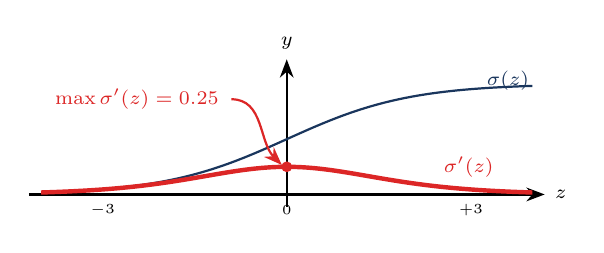
\begin{tikzpicture}[scale=0.78]
    \draw[-{Stealth}, thick] (-4.2, 0) -- (4.2, 0) node[right, font=\scriptsize] {$z$};
    \draw[-{Stealth}, thick] (0, -0.2) -- (0, 2.2) node[above, font=\scriptsize] {$y$};
    
    % Sigmoid curve: y = 1.8 / (1 + exp(-x))
    \draw[domain=-4:4, samples=50, smooth, thick, mainnavy] 
        plot (\x, {1.8 / (1.0 + exp(-\x))});
    \node[mainnavy, font=\scriptsize\bfseries, anchor=west] at (3.1, 1.85) {$\sigma(z)$};
    
    % Same vertical scale as sigmoid: max derivative 0.25 is drawn at 0.45.
    \draw[domain=-4:4, samples=50, smooth, ultra thick, crimsonred] 
        plot (\x, {1.8 * exp(-\x) / ((1.0 + exp(-\x))*(1.0 + exp(-\x)))});
    \node[crimsonred, font=\scriptsize\bfseries, anchor=west] at (2.4, 0.45) {$\sigma'(z)$};
    
    % Mark peak derivative cleanly in upper-left quadrant
    \fill[crimsonred] (0, 0.45) circle (2.5pt);
    \draw[-{Stealth}, crimsonred, thick] (-0.9, 1.55) to[out=0, in=135] (-0.08, 0.48);
    \node[crimsonred, font=\scriptsize\bfseries, anchor=east] at (-0.95, 1.55) {$\max \sigma'(z) = 0.25$};
    
    \node at (-3, -0.25) [font=\tiny] {$-3$};
    \node at (3, -0.25) [font=\tiny] {$+3$};
    \node at (0, -0.25) [font=\tiny] {$0$};
\end{tikzpicture}
\vspace{1pt}
\begin{block}{\textbf{Công thức Sigmoid \& Đạo hàm}}
\scriptsize
\textbf{Hàm kích hoạt}: $\sigma(z) = \dfrac{1}{1 + e^{-z}} \in (0, 1)$\\[2pt]
\textbf{Đạo hàm}: $\sigma'(z) = \sigma(z)(1 - \sigma(z)) \le \mathbf{0.25}$ (đạt cực đại tại $z=0$).
\end{block}
\end{column}

\begin{column}{0.50\textwidth}
\begin{alertblock}{\textbf{Hiệu ứng Nhân dồn Backpropagation}}
\scriptsize
\begin{itemize}\setlength{\itemsep}{2pt}
    \item Với chuỗi vô hướng $z_l=w_la_{l-1}+b_l$, $a_l=\sigma(z_l)$:
    $\frac{\partial \mathcal{L}}{\partial w_1} = \frac{\partial \mathcal{L}}{\partial a_L} a_0\sigma'(z_1) \prod_{l=2}^L w_l\sigma'(z_l)$
    \item Riêng tích 10 đạo hàm sigmoid không vượt quá:
    $$0.25^{10} \approx \mathbf{9.5 \times 10^{-7}} \approx \mathbf{0}!$$
    \item Khi mạng có nhiều tầng, chuỗi nhân dồn các giá trị nhỏ hơn $0.25$ khiến biên độ gradient suy giảm nhanh chóng về phía các tầng đầu.
\end{itemize}
\end{alertblock}

\begin{exampleblock}{\textbf{Giải pháp Phổ biến: Hàm Kích hoạt ReLU}}
\scriptsize
$\text{ReLU}(z) = \max(0, z) \to \text{ReLU}'(z) = \mathbf{1}$ với mọi $z > 0$.\\
Đạo hàm bằng $1$ trên miền dương giúp duy trì biên độ gradient ổn định khi truyền ngược qua các tầng sâu.
\end{exampleblock}
\end{column}
\end{columns}
\end{frame}

% SLIDE 21: GIẢI PHÁP 1: CHUẨN HÓA Z-SCORE
\begin{frame}{Giải pháp 1: Chuẩn hóa Dữ liệu Đầu vào (Z-Score Normalization)}
\begin{columns}[T]
\begin{column}{0.48\textwidth}
\begin{block}{\textbf{Công thức Chuẩn hóa Z-Score}}
\small
Với mỗi kênh, dùng $\mu,\sigma$ từ tập train hoặc theo yêu cầu của mô hình tiền huấn luyện:
$$x_{\text{norm}} = \frac{x - \mu}{\sigma}$$
\begin{itemize}\setlength{\itemsep}{2pt}
    \item Bộ thông số $(\mu, \sigma)$ tính toán từ tập huấn luyện (hoặc theo chuẩn ImageNet) được áp dụng nhất quán cho cả tập validation và test.
    \item \textbf{Thống kê ImageNet chuẩn (với giá trị RGB trong $[0,1]$)}:
    \begin{itemize}\setlength{\itemsep}{1pt}
        \item $\mu = [0.485, 0.456, 0.406]$
        \item $\sigma = [0.229, 0.224, 0.225]$
    \end{itemize}
\end{itemize}
\end{block}
\end{column}

\begin{column}{0.48\textwidth}
\begin{exampleblock}{\textbf{Tác động lên Loss Surface}}
\small
\begin{itemize}\setlength{\itemsep}{3pt}
    \item \textbf{Khi chưa chuẩn hóa}: Chênh lệch biên độ giữa các kênh khiến mặt cong mất mát bị kéo dẹt, quá trình gradient descent dễ bị dao động.
    \item \textbf{Sau khi chuẩn hóa}: Mặt cong trở nên cân đối hơn, giúp thuật toán tối ưu bước đi ổn định và hội tụ nhanh hơn.
\end{itemize}
\end{exampleblock}
\end{column}
\end{columns}
\end{frame}

% SLIDE 34 (MỚI): MINH HỌA TRỰC QUAN TÁC ĐỘNG CỦA Z-SCORE LÊN LOSS SURFACE
\begin{frame}{Minh họa Trực quan: Tác động của Z-Score lên Mặt cong Hàm mất mát}
\begin{columns}[T]
\begin{column}{0.48\textwidth}
\begin{alertblock}{\textbf{Chưa Chuẩn hóa: Thung lũng Elip Dẹt}}
\centering
\vspace{3pt}
\begin{tikzpicture}[scale=0.82]
    % Coordinate axes
    \draw[-{Stealth}, gray!70] (-2.6, 0) -- (2.6, 0) node[right, font=\tiny] {$w_1$};
    \draw[-{Stealth}, gray!70] (0, -1.6) -- (0, 1.6) node[above, font=\tiny] {$w_2$};
    
    % Elliptical contour lines
    \draw[thick, crimsonred!40] (0, 0) ellipse (2.3cm and 0.65cm);
    \draw[thick, crimsonred!60] (0, 0) ellipse (1.6cm and 0.45cm);
    \draw[thick, crimsonred!80] (0, 0) ellipse (0.95cm and 0.27cm);
    \draw[thick, crimsonred] (0, 0) ellipse (0.35cm and 0.10cm);
    \fill[crimsonred] (0, 0) circle (2pt);
    
    % Zigzag gradient path
    \draw[-{Stealth}, line width=1.3pt, crimsonred] (-2.1, 1.3) -- (-1.7, -0.55);
    \draw[-{Stealth}, line width=1.3pt, crimsonred] (-1.7, -0.55) -- (-1.1, 0.45);
    \draw[-{Stealth}, line width=1.3pt, crimsonred] (-1.1, 0.45) -- (-0.65, -0.35);
    \draw[-{Stealth}, line width=1.3pt, crimsonred] (-0.65, -0.35) -- (-0.25, 0.25);
    \draw[-{Stealth}, line width=1.3pt, crimsonred] (-0.25, 0.25) -- (0, 0);
    
    % Start point
    \fill[darkgray] (-2.1, 1.3) circle (2pt) node[above left, font=\tiny] {Khởi tạo};
    
    \node at (0, -1.35) [font=\scriptsize\bfseries, text=crimsonred] {Dao động Zigzag -- Rất khó hội tụ};
\end{tikzpicture}
\end{alertblock}
\vspace{-4pt}
\begin{block}{\textbf{Cơ chế Vật lý}}
\scriptsize
Tỷ lệ độ cong quá lệch giữa các chiều khiến gradient bật nảy qua lại giữa hai sườn dốc thay vì tiến thẳng về tâm.
\end{block}
\end{column}

\begin{column}{0.48\textwidth}
\begin{exampleblock}{\textbf{Sau Chuẩn hóa: Ví dụ Đơn giản}}
\centering
\vspace{3pt}
\begin{tikzpicture}[scale=0.82]
    % Coordinate axes
    \draw[-{Stealth}, gray!70] (-2.1, 0) -- (2.1, 0) node[right, font=\tiny] {$w_1$};
    \draw[-{Stealth}, gray!70] (0, -1.6) -- (0, 1.6) node[above, font=\tiny] {$w_2$};
    
    % Circular contour lines
    \draw[thick, accentteal!40] (0, 0) circle (1.5cm);
    \draw[thick, accentteal!60] (0, 0) circle (1.05cm);
    \draw[thick, accentteal!80] (0, 0) circle (0.65cm);
    \draw[thick, accentteal] (0, 0) circle (0.25cm);
    \fill[accentteal] (0, 0) circle (2pt);
    
    % Direct gradient path
    \draw[-{Stealth}, line width=1.3pt, accentteal] (-1.3, 1.2) -- (-0.65, 0.6);
    \draw[-{Stealth}, line width=1.3pt, accentteal] (-0.65, 0.6) -- (0, 0);
    
    % Start point
    \fill[darkgray] (-1.3, 1.2) circle (2pt) node[above left, font=\tiny] {Khởi tạo};
    
    \node at (0, -1.35) [font=\scriptsize\bfseries, text=accentteal] {Đường hội tụ trong ví dụ minh họa};
\end{tikzpicture}
\end{exampleblock}
\vspace{-4pt}
\begin{block}{\textbf{Ý nghĩa Tối ưu}}
\scriptsize
Chuẩn hóa dữ liệu đầu vào giúp cải thiện điều kiện hình học của hàm mất mát, giảm thiểu hiện tượng dao động qua lại và tăng tính ổn định của các bước cập nhật trọng số.
\end{block}
\end{column}
\end{columns}
\end{frame}

% SLIDE 23: GIẢI PHÁP 3: BATCH NORMALIZATION (BN)
\begin{frame}{Giải pháp 2: Kỹ thuật Chuẩn hóa theo Lô (Batch Normalization)}
\begin{columns}[T]
\begin{column}{0.48\textwidth}
\begin{block}{\textbf{4 Bước Tính toán của Tầng BN}}
\scriptsize
Xét một kênh: $\mathcal{B} = \{x_1, \dots, x_m\}$. Với BN2d, $m=N\times H\times W$:
\begin{align*}
\mu_{\mathcal{B}} &= \frac{1}{m} \sum_{i=1}^{m} x_i \quad (\text{Trung bình lô}) \\
\sigma_{\mathcal{B}}^2 &= \frac{1}{m} \sum_{i=1}^{m} (x_i - \mu_{\mathcal{B}})^2 \quad (\text{Phương sai lô}) \\
\hat{x}_i &= \frac{x_i - \mu_{\mathcal{B}}}{\sqrt{\sigma_{\mathcal{B}}^2 + \epsilon}} \quad (\text{Chuẩn hóa}) \\
y_i &= \gamma \hat{x}_i + \beta \quad (\text{Khôi phục Biểu diễn})
\end{align*}
Mỗi kênh có hai tham số học được $\gamma,\beta$. Khi suy luận, BN mặc định dùng trung bình và phương sai tích lũy khi train.
\end{block}
\end{column}

\begin{column}{0.48\textwidth}
\begin{exampleblock}{\textbf{3 Tác động Chính của Batch Normalization}}
\small
\begin{enumerate}\setlength{\itemsep}{3pt}
    \item \textbf{Ổn định phân phối kích hoạt}: Giảm thiểu sự trôi dạt phân phối nội tại (internal covariate shift) giữa các tầng qua từng bước học.
    \item \textbf{Hỗ trợ tốc độ học lớn hơn}: Cải thiện dòng chảy gradient, cho phép thiết lập tốc độ học (learning rate) lớn hơn mà vẫn ổn định.
    \item \textbf{Tác dụng điều chuẩn nhẹ}: Sự biến thiên ngẫu nhiên của thống kê trên từng mini-batch tạo ra hiệu ứng làm mịn tự nhiên, hạn chế quá khớp.
\end{enumerate}
\end{exampleblock}
\end{column}
\end{columns}
\end{frame}

% SLIDE 25: GIẢI PHÁP 5: ĐỘT PHÁ SKIP CONNECTION (RESNET)
\begin{frame}{Giải pháp 3: Kỹ thuật Kết nối Tắt (Skip Connection / Residual)}
\begin{columns}[T]
\begin{column}{0.48\textwidth}
\centering
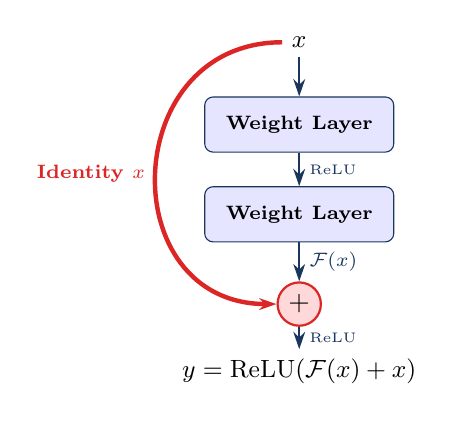
\begin{tikzpicture}[
    scale=0.95,
    box/.style={rectangle, draw=mainnavy, fill=blue!10, rounded corners=3pt, minimum width=2.4cm, minimum height=0.7cm, font=\scriptsize\bfseries, align=center},
    addnode/.style={circle, draw=crimsonred, fill=red!15, thick, inner sep=1pt, minimum size=0.55cm, font=\normalsize\bfseries}
]
    \node (x) at (0, 3.4) [font=\small\bfseries] {$x$};
    \node[box] (c1) at (0, 2.3) {Weight Layer};
    \node[box] (c2) at (0, 1.1) {Weight Layer};
    \node[addnode] (add) at (0, -0.1) {$+$};
    \node (out) at (0, -1.0) [font=\small\bfseries] {$y = \mathrm{ReLU}(\mathcal{F}(x) + x)$};

    \draw[flowarrow] (x) -- (c1);
    \draw[flowarrow] (c1) -- (c2) node[midway, right, font=\tiny] {ReLU};
    \draw[flowarrow] (c2) -- (add) node[midway, right, font=\scriptsize] {$\mathcal{F}(x)$};
    \draw[flowarrow] (add) -- (out) node[midway, right, font=\tiny] {ReLU};

    % Skip arrow
    \draw[flowarrow_red, ultra thick] (x) to[out=180, in=180, looseness=1.6] node[midway, left, font=\scriptsize\bfseries] {Identity $x$} (add);
\end{tikzpicture}
\end{column}

\begin{column}{0.48\textwidth}
\begin{block}{\textbf{Học Phần Thặng dư (Residual Learning)}}
\small
\begin{itemize}\setlength{\itemsep}{2.5pt}
    \item Thay vì ép các tầng tích chập phải học toàn bộ ánh xạ mục tiêu $\mathcal{H}(x)$, ResNet tái cấu trúc để mạng học phần sai khác (thặng dư):
    $$\mathcal{F}(x) = \mathcal{H}(x) - x \implies \mathcal{H}(x) = \mathcal{F}(x) + x$$
    \item \textbf{Trực giác Tối ưu}: Nếu việc tăng tầng không mang lại biểu diễn tốt hơn, mạng có thể dễ dàng triệt tiêu $\mathcal{F}(x) \to 0$ để giữ lại ánh xạ đồng nhất (identity mapping).
    \item \textbf{Đảm bảo Tương thích}: Nhánh tắt yêu cầu kích thước tensor của $\mathcal{F}(x)$ và $x$ phải đồng nhất; khi giảm chiều không gian hoặc thay đổi số kênh, sử dụng phép chiếu $1\times 1$ conv thích hợp.
\end{itemize}
\end{block}
\end{column}
\end{columns}
\end{frame}

% SLIDE 26: BẢN CHẤT TOÁN HỌC: ĐẠI LỘ GRADIENT
\begin{frame}{Bản chất Toán học: Đại lộ Gradient (Gradient Highway)}
\begin{columns}[T]
\begin{column}{0.48\textwidth}
\begin{alertblock}{\textbf{Chứng minh Toán học}}
\small
Xét nhánh tắt đồng nhất, không có kích hoạt sau phép cộng; viết cho trường hợp vô hướng:
$$x_{l+1} = x_l + \mathcal{F}(x_l, \mathcal{W}_l)$$
Mở rộng đệ quy lên tầng $L > l$:
$$x_L = x_l + \sum_{i=l}^{L-1} \mathcal{F}(x_i, \mathcal{W}_i)$$
Đạo hàm tổn thất $\mathcal{L}$ theo $x_l$:
$$\frac{\partial \mathcal{L}}{\partial x_l} = \frac{\partial \mathcal{L}}{\partial x_L} \cdot \frac{\partial x_L}{\partial x_l} = \frac{\partial \mathcal{L}}{\partial x_L} \left( \mathbf{1} + \frac{\partial}{\partial x_l} \sum_{i=l}^{L-1} \mathcal{F}(x_i, \mathcal{W}_i) \right)$$
\end{alertblock}
\end{column}

\begin{column}{0.48\textwidth}
\begin{exampleblock}{\textbf{Ý nghĩa Cốt lõi của Số hạng $+1$}}
\small
\begin{itemize}\setlength{\itemsep}{3pt}
    \item Số hạng $\mathbf{+1}$ tạo ra đường truyền gradient trực tiếp từ tầng sâu về tầng nông, hạn chế sự suy giảm qua các chuỗi nhân liên tiếp.
    \item Ngay cả khi gradient qua nhánh dư $\mathcal{F}$ tiến về 0, tín hiệu đạo hàm vẫn được dẫn truyền thông suốt qua nhánh tắt đồng nhất.
    \item \textbf{Mở rộng độ sâu}: Tạo tiền đề cho việc thiết kế và huấn luyện thành công các mạng nơ-ron sâu như ResNet-50, ResNet-101 và ResNet-152.
\end{itemize}
\end{exampleblock}
\end{column}
\end{columns}
\end{frame}

% =============================================================
% PHẦN 5: KIỂM SOÁT QUÁ KHỚP & BỘ VŨ KHÍ ĐIỀU CHUẨN (SLIDES 27 - 30)
% =============================================================

% SLIDE 27: THÁCH THỨC QUÁ KHỚP & GENERALIZATION GAP
\begin{frame}{Thách thức 2: Quá khớp (Overfitting) \& Generalization Gap}
\begin{columns}[T]
\begin{column}{0.48\textwidth}
\begin{block}{\textbf{Bản chất Hiện tượng Quá khớp}}
\small
\begin{itemize}\setlength{\itemsep}{3pt}
    \item Mạng nơ-ron sâu có dung lượng học (Capacity) rất lớn, dễ dàng khớp hoàn hảo cả các nhiễu ngẫu nhiên trong tập huấn luyện.
    \item \textbf{Triệu chứng Điển hình}:
    \begin{itemize}\setlength{\itemsep}{2pt}
        \item Train Loss tiếp tục giảm sâu tiệm cận 0.
        \item Validation Loss bắt đầu phân kỳ và tăng vọt sau một số epochs nhất định.
    \end{itemize}
\end{itemize}
\end{block}
\end{column}

\begin{column}{0.48\textwidth}
\begin{alertblock}{\textbf{Khoảng cách Tổng quát hóa (Gap)}}
\small
$$\text{Generalization Gap} = \text{Accuracy}_{\text{Train}} - \text{Accuracy}_{\text{Val}}$$
\begin{itemize}\setlength{\itemsep}{2pt}
    \item \textbf{Mục tiêu kiểm soát}: Đánh giá sự khác biệt giữa hiệu năng trên tập huấn luyện và tập kiểm định. Một mô hình có độ tổng quát hóa tốt cần thu hẹp khoảng cách Gap, đồng thời duy trì độ chính xác cao trên tập kiểm định.
\end{itemize}
\end{alertblock}
\end{column}
\end{columns}
\end{frame}

% SLIDE 28: BỘ 5 VŨ KHÍ ĐIỀU CHUẨN
\begin{frame}{5 Kỹ thuật Điều chuẩn và Tối ưu Huấn luyện}
\begin{columns}[T]
\begin{column}{0.48\textwidth}
\begin{block}{\textbf{1. Tăng cường Dữ liệu (Data Augmentation)}}
\scriptsize
Random Crop ($32\times 32$, pad 4), Random Horizontal Flip ($p=0.5$), ColorJitter. Tạo dữ liệu mới nhân tạo, ngăn mô hình nhớ vị trí pixel tuyệt đối.
\end{block}

\begin{block}{\textbf{2. Chuẩn hóa theo Lô (Batch Normalization)}}
\scriptsize
Chuẩn hóa kích hoạt ở từng tầng, đồng thời tạo nhiễu ngẫu nhiên nhẹ giữa các mini-batch giúp tăng cường độ ổn định.
\end{block}

\begin{block}{\textbf{3. Inverted Dropout ($p=0.2\text{--}0.5$)}}
\scriptsize
Khi train, đặt mỗi kích hoạt về 0 với xác suất $p$ (20--50\%); phần còn lại nhân $1/(1-p)$. Khi eval, tắt dropout. Cách này giúp giảm sự phụ thuộc lẫn nhau giữa các nơ-ron.
\end{block}
\end{column}

\begin{column}{0.48\textwidth}
\begin{block}{\textbf{4. Suy giảm Trọng số (Weight Decay / $L_2$)}}
\scriptsize
Phạt các trọng số có độ lớn quá cao:
$$\mathcal{L}_{\text{total}} = \mathcal{L}_{\text{CE}} + \frac{\lambda}{2} \|W\|_2^2$$
Phạt độ lớn của ma trận trọng số, khuyến khích mô hình duy trì trọng số nhỏ và phân bổ mượt mà, hạn chế phụ thuộc cục bộ vào một số đặc trưng riêng lẻ.
\end{block}

\begin{block}{\textbf{5. Cosine Annealing Learning Rate}}
\scriptsize
Điều chỉnh tốc độ học giảm dần theo đồ thị cosine kết hợp Warmup ở giai đoạn đầu, giúp mô hình hội tụ mượt mà và tìm được các vùng cực tiểu ổn định hơn.
\end{block}
\end{column}
\end{columns}
\end{frame}

% SLIDE 29: ABLATION STUDY THỰC NGHIỆM
\begin{frame}{Nghiên cứu Bóc tách Thực nghiệm (Ablation Study) trên CIFAR-10}
\begin{table}
\centering
\resizebox{0.96\textwidth}{!}{%
\begin{tabular}{lcccc}
\toprule
\textbf{Cấu hình Thử nghiệm} & \textbf{Train Acc} & \textbf{Val Acc} & \textbf{Gap (điểm \%)} & \textbf{Tăng Val (điểm \%)} \\
\midrule
1. Baseline CNN (Không điều chuẩn) & $99.2\%$ & $78.4\%$ & \alert{$20.8$} & Điểm mốc cơ sở (Overfit) \\
2. + Batch Normalization & $99.8\%$ & $84.5\%$ & $15.3$ & $+6.1$ (Ổn định gradient) \\
3. + Inverted Dropout ($p=0.3$) & $99.2\%$ & $86.2\%$ & $13.0$ & $+1.7$ (Chống co-adaptation) \\
4. + Weight Decay ($10^{-4}$ AdamW) & $95.2\%$ & $87.5\%$ & $7.7$ & $+1.3$ (Phạt biên độ lớn) \\
5. + Data Augmentation \& LR Scheduler & $98.1\%$ & $90.7\%$ & $7.4$ & $+3.2$ (Tăng đa dạng mẫu) \\
\textbf{6. + Skip Connection (ResNet)} & $\mathbf{98.3\%}$ & $\mathbf{94.5\%}$ & $\mathbf{3.8}$ & $\mathbf{+3.8}$ (Đại lộ Gradient) \\
\bottomrule
\end{tabular}%
}
\end{table}

\begin{block}{\textbf{Phân tích Kết quả Thực nghiệm}}
\scriptsize
\begin{itemize}\setlength{\itemsep}{2pt}
    \item \textbf{Hiệu quả tích lũy}: Việc kết hợp đồng bộ các kỹ thuật chuẩn hóa, điều chuẩn và lịch học giúp thu hẹp khoảng cách Gap từ $20.8\%$ xuống còn $3.8\%$, đồng thời nâng Val Accuracy từ $78.4\%$ lên $94.5\%$.
    \item \textbf{Ý nghĩa thực nghiệm}: Mỗi cải tiến cấu trúc đóng góp tích cực vào việc hạn chế hiện tượng quá khớp và cải thiện độ chính xác tổng quát hóa trên CIFAR-10.
\end{itemize}
\end{block}
\end{frame}

% SLIDE: CÀI ĐẶT PYTORCH MÔ HÌNH CNN + ĐIỀU CHUẨN & SKIP CONNECTION
\begin{frame}{Thực nghiệm: Cài đặt PyTorch CNN Điều chuẩn \& Skip Connection}
\centering
\includegraphics[width=0.96\textwidth,height=0.82\textheight,keepaspectratio]{figures/crop_slide_cifar10_regularization_skip_code.png}
\end{frame}

% SLIDE 30: MINH CHỨNG NOTEBOOK GENERALIZATION
\begin{frame}{Minh chứng Thực nghiệm Notebook: Đối sánh Generalization}
\begin{columns}[T]
\begin{column}{0.62\textwidth}
\centering
\includegraphics[width=0.98\textwidth]{figures/fig_generalization_empirical.png}
\end{column}

\begin{column}{0.36\textwidth}
\begin{alertblock}{\textbf{Mô hình Baseline (Chưa điều chuẩn)}}
\scriptsize
\begin{itemize}\setlength{\itemsep}{2pt}
    \item Đường cong Train và Test nhanh chóng tách xa nhau sau các epoch đầu.
    \item Train đạt gần $99\%$ trong khi Test dừng ở mức $\approx 78\%$, phản ánh sự chênh lệch đáng kể do hiện tượng quá khớp.
\end{itemize}
\end{alertblock}

\begin{exampleblock}{\textbf{Mô hình Điều chuẩn \& Skip Connection}}
\scriptsize
\begin{itemize}\setlength{\itemsep}{2pt}
    \item Hai đường cong Train và Test tiến sát nhau và cùng tăng trưởng ổn định.
    \item Đạt độ chính xác kiểm định $\approx 94.5\%$, khoảng cách chênh lệch được thu hẹp rõ rệt, chứng minh hiệu quả tổng quát hóa thực tế.
\end{itemize}
\end{exampleblock}
\end{column}
\end{columns}
\end{frame}

% =============================================================
% PHẦN 6: BIÊN NIÊN SỬ TIẾN HÓA KIẾN TRÚC -- SỢI CHỈ ĐỎ DẪN DẮT (SLIDES 31 - 35)
% =============================================================

% SLIDE 31: TRỤC THỜI GIAN 25 NĂM
\begin{frame}{Dòng thời gian 25 năm \& Sợi chỉ đỏ Tiến hóa Kiến trúc}
\centering
\begin{tikzpicture}[
    scale=0.92,
    yearnode/.style={circle, draw=mainnavy, fill=blue!15, thick, font=\tiny\bfseries, inner sep=1pt, minimum size=0.65cm},
    boxdesc/.style={rectangle, draw=slate!50, fill=lightbg, rounded corners=3pt, font=\tiny, align=center, inner sep=4pt}
]
    % Timeline horizontal axis
    \draw[-{Stealth[length=3mm]}, ultra thick, mainnavy] (0, 0) -- (12.5, 0);

    % Milestones
    % 1998 LeNet
    \node[yearnode] (y98) at (0.8, 0) {1998};
    \node[boxdesc, above=0.35cm of y98] {\textbf{LeNet-5}\\Conv + Subsampling\\Chữ số viết tay};
    \draw[thick, mainnavy] (y98) -- (0.8, 0.35);

    % 2012 AlexNet
    \node[yearnode] (y12) at (2.8, 0) {2012};
    \node[boxdesc, below=0.35cm of y12] {\textbf{AlexNet}\\8 Tầng, GPU, ReLU\\Cách mạng Deep Learning};
    \draw[thick, mainnavy] (y12) -- (2.8, -0.35);

    % 2014 VGG / GoogLeNet
    \node[yearnode] (y14) at (4.8, 0) {2014};
    \node[boxdesc, above=0.35cm of y14] {\textbf{VGG \& Inception}\\VGG: Kernel $3\times 3$\\Inception: Đa nhánh};
    \draw[thick, mainnavy] (y14) -- (4.8, 0.35);

    % 2015 ResNet
    \node[yearnode] (y15) at (6.8, 0) {2015};
    \node[boxdesc, below=0.35cm of y15] {\textbf{ResNet-152}\\Skip Connection\\Thắng ILSVRC 2015};
    \draw[thick, mainnavy] (y15) -- (6.8, -0.35);

    % 2017 MobileNet
    \node[yearnode] (y17) at (8.6, 0) {2017};
    \node[boxdesc, above=0.35cm of y17] {\textbf{MobileNet v1 (2017)}\\\textbf{v2 (2018)}\\Tinh gọn cho Edge AI};
    \draw[thick, mainnavy] (y17) -- (8.6, 0.35);

    % 2020 ViT
    \node[yearnode] (y20) at (10.2, 0) {2020};
    \node[boxdesc, below=0.35cm of y20] {\textbf{Vision Transformer}\\Self-Attention\\Đe dọa soán ngôi CNN};
    \draw[thick, mainnavy] (y20) -- (10.2, -0.35);

    % 2022 ConvNeXt
    \node[yearnode] (y22) at (11.8, 0) {2022};
    \node[boxdesc, above=0.35cm of y22] {\textbf{ConvNeXt}\\Hiện đại hóa CNN\\Cạnh tranh với Swin};
    \draw[thick, mainnavy] (y22) -- (11.8, 0.35);
\end{tikzpicture}

\vspace{6pt}
\begin{block}{\textbf{Quy luật Tiến hóa Đúc kết}}
\scriptsize
Mỗi thế hệ kiến trúc phát triển là bước tiến giải quyết các thách thức kỹ thuật của thế hệ trước:
$$\text{Nông (LeNet)} \xrightarrow{\text{GPU+ReLU}} \text{Sâu (AlexNet)} \xrightarrow{3\times 3} \text{Kernel nhỏ (VGG)} \xrightarrow{\text{Residual}} \text{Siêu sâu (ResNet)} \xrightarrow{\text{Separable}} \text{Di động (MobileNet)} \xrightarrow{\text{Modern}} \text{ConvNeXt}$$
\end{block}
\end{frame}

% =============================================================
% SLIDE 42: ĐỘT PHÁ 1: VGGNET
% =============================================================
\begin{frame}{Kiến trúc 1: Thừa số hóa Kernel \& Chuỗi Tích chập $3\times 3$ (VGGNet)}
\begin{columns}[T]
\begin{column}{0.48\textwidth}
\centering
\vspace{2pt}
\begin{tikzpicture}[scale=0.82]
    % Input grid (7 elements)
    \foreach \x in {0,...,6} {
        \draw[fill=blue!8, draw=mainnavy!50] (\x*0.65, 0) rectangle ++(0.65, 0.45);
        \node at (\x*0.65+0.325, 0.225) [font=\tiny] {$x_{\x}$};
    }
    \node at (-0.6, 0.225) [font=\scriptsize\bfseries, text=mainnavy] {Đầu vào};
    \draw[decorate, decoration={brace, mirror, amplitude=4pt}] (0, -0.08) -- (4.55, -0.08) node[midway, below=4pt, font=\tiny\bfseries] {Vùng nhìn $7\times 7$};

    % Conv Layer 1 (5 elements)
    \foreach \x in {0,...,4} {
        \draw[fill=orange!15, draw=warmorange!80] (\x*0.65+0.65, 1.3) rectangle ++(0.65, 0.45);
    }
    \node at (-0.6, 1.525) [font=\scriptsize\bfseries, text=warmorange] {Tầng 1 ($3\times 3$)};
    \draw[thin, gray!70] (0, 0.45) -- (0.65, 1.3);
    \draw[thin, gray!70] (1.95, 0.45) -- (1.30, 1.3);

    % Conv Layer 2 (3 elements)
    \foreach \x in {0,...,2} {
        \draw[fill=teal!15, draw=accentteal!80] (\x*0.65+1.3, 2.6) rectangle ++(0.65, 0.45);
    }
    \node at (-0.6, 2.825) [font=\scriptsize\bfseries, text=accentteal] {Tầng 2 ($3\times 3$)};
    \draw[thin, gray!70] (0.65, 1.75) -- (1.30, 2.6);
    \draw[thin, gray!70] (2.60, 1.75) -- (1.95, 2.6);

    % Conv Layer 3 (1 element)
    \draw[fill=emeraldgreen!20, draw=emeraldgreen, thick] (1.95, 3.9) rectangle ++(0.65, 0.45);
    \node at (2.275, 4.125) [font=\tiny\bfseries] {$y$};
    \node at (-0.6, 4.125) [font=\scriptsize\bfseries, text=emeraldgreen] {Tầng 3 ($3\times 3$)};
    \draw[thick, emeraldgreen] (1.30, 3.05) -- (1.95, 3.9);
    \draw[thick, emeraldgreen] (3.25, 3.05) -- (2.60, 3.9);

    \node at (2.275, 4.65) [font=\scriptsize\bfseries, text=mainnavy] {1 Nơ-ron nhìn trọn vùng $7\times 7$!};
\end{tikzpicture}
\end{column}

\begin{column}{0.50\textwidth}
\begin{block}{\textbf{Bản chất Hình học \& Tối ưu Tham số}}
\footnotesize
\begin{itemize}\setlength{\itemsep}{2.5pt}
    \item \textbf{Tương đương Trường Tiếp nhận}: Chuỗi 3 tầng $3\times 3$ liên tiếp (stride 1) bao quát vùng nhìn hiệu dụng đúng bằng 1 tầng $7\times 7$ ($1 + 3 \times (3-1) = 7$).
    \item \textbf{Tiết kiệm Tham số}: Với cùng số kênh $C$, tỷ lệ trọng số giữa hai cách tiếp cận:
    $$\text{Tỷ lệ} = \frac{3 \times (3^2 \cdot C^2)}{1 \times (7^2 \cdot C^2)} = \frac{27}{49} \approx \mathbf{55\%}$$
    Giúp giảm khoảng \textbf{45\% số lượng trọng số} cần học.
    \item \textbf{Tăng cường Tính Phi tuyến}: Bổ sung 3 hàm kích hoạt ReLU xen kẽ thay vì chỉ 1, giúp mạng học được các biểu diễn đặc trưng phong phú hơn.
\end{itemize}
\end{block}

\vspace{-1pt}
\begin{exampleblock}{\textbf{Đóng góp cho Thiết kế CNN}}
\scriptsize
Nguyên lý xếp chồng các kernel nhỏ $3\times 3$ trở thành tiêu chuẩn nền tảng cho phần lớn các kiến trúc mạng hiện đại sau này.
\end{exampleblock}
\end{column}
\end{columns}
\end{frame}

% =============================================================
% SLIDE 43: GOOGLENET INCEPTION (RỘNG RÃI, KHÔNG DÍNH NHAU)
% =============================================================
\begin{frame}{Kiến trúc 2: Khối Inception Đa Quy mô \& Nút thắt $1\times 1$ (GoogLeNet)}
\begin{columns}[T]
\begin{column}{0.54\textwidth}
\centering
\vspace{1pt}
\begin{tikzpicture}[
    basebox/.style={rectangle, draw=mainnavy, fill=blue!10, rounded corners=3pt, font=\scriptsize\bfseries, align=center, minimum width=7.2cm, minimum height=0.52cm},
    nbox/.style={rectangle, draw=mainnavy!80, fill=blue!8, rounded corners=2pt, font=\scriptsize\bfseries, align=center, minimum width=1.35cm, minimum height=0.55cm},
    botbox/.style={rectangle, draw=warmorange!90, fill=warmorange!20, rounded corners=2pt, font=\scriptsize\bfseries, align=center, minimum width=1.35cm, minimum height=0.55cm},
    catbox/.style={rectangle, draw=accentteal, fill=teal!18, rounded corners=3pt, font=\scriptsize\bfseries, align=center, minimum width=7.2cm, minimum height=0.52cm}
]
    % Input block at y = 0.0, width 7.2cm
    \node[basebox] (prev) at (0, 0.0) {Đầu vào Khối (Feature Map từ tầng trước)};

    % 4 Branches at x = -2.7, -0.9, +0.9, +2.7 (Spacing = 1.8cm, Box width = 1.35cm -> Gap = 0.45cm!)
    % Branch 1: Conv 1x1 (centered vertically at y = 2.1)
    \node[nbox] (b1) at (-2.7, 2.1) {Conv\\$1\times 1$};

    % Branch 2: Conv 1x1 (Nén) -> Conv 3x3
    \node[botbox] (b2_1) at (-0.9, 1.3) {Conv $1\times 1$\\{\fontsize{5.5}{6}\selectfont(Nén)}};
    \node[nbox] (b2_2) at (-0.9, 2.9) {Conv\\$3\times 3$};

    % Branch 3: Conv 1x1 (Nén) -> Conv 5x5
    \node[botbox] (b3_1) at (0.9, 1.3) {Conv $1\times 1$\\{\fontsize{5.5}{6}\selectfont(Nén)}};
    \node[nbox] (b3_2) at (0.9, 2.9) {Conv\\$5\times 5$};

    % Branch 4: MaxPool 3x3 -> Conv 1x1 (Nén)
    \node[nbox] (b4_1) at (2.7, 1.3) {MaxPool\\$3\times 3$};
    \node[botbox] (b4_2) at (2.7, 2.9) {Conv $1\times 1$\\{\fontsize{5.5}{6}\selectfont(Nén)}};

    % Output block at y = 4.0, width 7.2cm
    \node[catbox] (concat) at (0, 4.0) {Ghép Kênh theo Chiều sâu (DepthConcat)};

    % Arrows from Input
    \draw[flowarrow] (-2.7, 0.26) -- (b1.south);
    \draw[flowarrow] (-0.9, 0.26) -- (b2_1.south);
    \draw[flowarrow] (b2_1) -- (b2_2);
    \draw[flowarrow] (0.9, 0.26) -- (b3_1.south);
    \draw[flowarrow] (b3_1) -- (b3_2);
    \draw[flowarrow] (2.7, 0.26) -- (b4_1.south);
    \draw[flowarrow] (b4_1) -- (b4_2);

    % Arrows to Output
    \draw[flowarrow_teal] (b1.north) -- (-2.7, 3.74);
    \draw[flowarrow_teal] (b2_2.north) -- (-0.9, 3.74);
    \draw[flowarrow_teal] (b3_2.north) -- (0.9, 3.74);
    \draw[flowarrow_teal] (b4_2.north) -- (2.7, 3.74);
\end{tikzpicture}

\vspace{4pt}
\begin{exampleblock}{\textbf{Cốt lõi Đột phá Hình học}}
\scriptsize
\textbf{4 Nhánh Đa quy mô}: Bắt trọn đặc trưng từ chi tiết nhỏ đến ngữ cảnh lớn. Nút thắt $1\times 1$ nén kênh giúp giảm tải tính toán trước các kernel lớn $3\times 3, 5\times 5$.
\end{exampleblock}
\end{column}

\begin{column}{0.44\textwidth}
\begin{block}{\textbf{Ý tưởng 1: Đa Quy mô Song song}}
\scriptsize
\begin{itemize}\setlength{\itemsep}{2pt}
    \item Thay vì đoán cỡ kernel, Inception \textbf{chạy song song cả ba}:
    \begin{itemize}\setlength{\itemsep}{1pt}
        \item $1\times 1$: Trộn thông tin kênh tại từng vị trí.
        \item $3\times 3$: Bắt chi tiết kích thước vừa.
        \item $5\times 5$: Bắt bối cảnh không gian lớn.
    \end{itemize}
    \item Ghép kênh rồi học cách kết hợp ở các tầng sau.
\end{itemize}
\end{block}

\vspace{-1pt}
\begin{alertblock}{\textbf{Ý tưởng 2: Nút thắt $1\times 1$ (Bottleneck)}}
\footnotesize
\begin{itemize}\setlength{\itemsep}{2pt}
    \item \textbf{Vấn đề}: Conv $5\times 5$ trên 256 kênh ngốn tính toán rất lớn.
    \item \textbf{Giải pháp}: Dùng Conv $1\times 1$ nén 256 kênh về 32 kênh trước khi qua $5\times 5$.
    \item \textbf{Hiệu quả tham số}: Nhờ kỹ thuật nén kênh và GAP, toàn bộ mạng GoogLeNet chỉ cần khoảng $6.8\text{M}$ tham số mà vẫn đạt độ chính xác cao.
\end{itemize}
\end{alertblock}
\end{column}
\end{columns}
\end{frame}

% =============================================================
% SLIDE 44: MOBILENET (TRỰC QUAN HÓA 3 LÀN KÊNH + POINTWISE)
% =============================================================
\begin{frame}{Kiến trúc 3: Tích chập Tách rời Không gian và Kênh (MobileNet Family)}
\begin{columns}[T]
\begin{column}{0.50\textwidth}
\centering
\begin{tikzpicture}[
    chbox/.style={rectangle, draw=mainnavy, fill=blue!12, rounded corners=2pt, font=\tiny\bfseries, align=center, minimum width=1.4cm, minimum height=0.45cm},
    kbox/.style={rectangle, draw=warmorange, fill=orange!20, rounded corners=2pt, font=\tiny\bfseries, align=center, minimum width=1.4cm, minimum height=0.45cm},
    pwbox/.style={rectangle, draw=accentteal, fill=teal!18, rounded corners=3pt, font=\scriptsize\bfseries, align=center, minimum width=5.8cm, minimum height=0.55cm}
]
    % Input Header
    \node (in) at (0, 4.4) [font=\scriptsize\bfseries, text=mainnavy] {Đầu vào Tensor $C_{\text{in}}$ kênh ($H \times W \times C_{\text{in}}$)};
    
    % Step 1: Depthwise Lane
        % Step 1: Depthwise Lane - separated with clean distance & brace
    \draw[decorate, decoration={brace, amplitude=4pt}, warmorange, line width=1pt] (-2.68, 1.7) -- (-2.68, 4.05);
    \node at (-3.15, 2.875) [font=\tiny\bfseries, text=warmorange, rotate=90] {BƯỚC 1: DEPTHWISE};
    
    % 3 Channels
    \node[chbox] (c1) at (-1.8, 3.8) {Kênh 1};
    \node[chbox] (c2) at (0.0, 3.8) {Kênh 2};
    \node[chbox] (c3) at (1.8, 3.8) {Kênh $C_{\text{in}}$};
    
    % 3 Filters
    \node[kbox] (k1) at (-1.8, 2.9) {Kernel $3\times 3$};
    \node[kbox] (k2) at (0.0, 2.9) {Kernel $3\times 3$};
    \node[kbox] (k3) at (1.8, 2.9) {Kernel $3\times 3$};

    % Feature maps out of Depthwise
    \node[chbox, fill=orange!10, draw=warmorange] (m1) at (-1.8, 2.0) {Map 1};
    \node[chbox, fill=orange!10, draw=warmorange] (m2) at (0.0, 2.0) {Map 2};
    \node[chbox, fill=orange!10, draw=warmorange] (m3) at (1.8, 2.0) {Map $C_{\text{in}}$};

    % Arrows in Step 1
    \draw[flowarrow] (-1.8, 4.2) -- (c1);
    \draw[flowarrow] (0.0, 4.2) -- (c2);
    \draw[flowarrow] (1.8, 4.2) -- (c3);

    \draw[flowarrow_orange] (c1) -- (k1);
    \draw[flowarrow_orange] (c2) -- (k2);
    \draw[flowarrow_orange] (c3) -- (k3);

    \draw[flowarrow_orange] (k1) -- (m1);
    \draw[flowarrow_orange] (k2) -- (m2);
    \draw[flowarrow_orange] (k3) -- (m3);

    % Step 2: Pointwise
    \node[pwbox] (pw) at (0, 0.9) {BƯỚC 2: Pointwise Conv ($1\times 1$)\\Tổ hợp tuyến tính trộn tất cả các kênh lại};
    
    \draw[flowarrow_teal] (m1.south) -- (-1.8, 1.25);
    \draw[flowarrow_teal] (m2.south) -- (0.0, 1.25);
    \draw[flowarrow_teal] (m3.south) -- (1.8, 1.25);

    % Output
    \node (out) at (0, 0.05) [font=\scriptsize\bfseries, text=accentteal] {Đầu ra: $H \times W \times C_{\text{out}}$ (Đầy đủ tương quan kênh)};
    \draw[flowarrow_teal] (pw) -- (out);
\end{tikzpicture}

\vspace{-5pt}
\begin{block}{\textbf{Hiệu quả Cắt giảm Chi phí Tính toán}}
\footnotesize
$$\text{Tỷ lệ FLOPs} = \frac{K^2M+MN}{K^2MN}=\frac{1}{N}+\frac{1}{K^2}\approx\frac{1}{9}$$
Với $K=3$ và số kênh $C_{out}$ đủ lớn, chi phí tính toán của khối tích chập giảm gần 8 đến 9 lần so với tích chập tiêu chuẩn.
\end{block}
\end{column}

\begin{column}{0.48\textwidth}
\begin{exampleblock}{\textbf{Đột phá Inverted Residual (MobileNetV2)}}
\footnotesize
\begin{itemize}\setlength{\itemsep}{3pt}
    \item \textbf{Cơ chế Phình Kênh Đảo ngược}:
    \begin{itemize}\setlength{\itemsep}{1.5pt}
        \item \textbf{ResNet (bottleneck)}: Kênh Dày $\to$ Nén Mỏng $\to$ Kênh Dày
        \item \textbf{MobileNetV2}: Kênh Mỏng $\to$ \textbf{Phình $6\times$} $\to$ Kênh Mỏng
    \end{itemize}
    \item \textbf{Mục đích}: Mở rộng không gian kênh trước phép kích hoạt phi tuyến giúp bảo toàn tốt hơn các đặc trưng biểu diễn.
    \item \textbf{Linear Bottleneck}: Giữ tuyến tính ở tầng nén mỏng cuối cùng nhằm tránh mất mát tín hiệu trên không gian số chiều thấp.
    \item \textbf{Skip Connection}: Kết nối tắt giữa các tầng nút thắt cùng số kênh, hỗ trợ lan truyền gradient hiệu quả.
    \item \textbf{Ứng dụng mục tiêu}: Thiết kế tối ưu cho các thiết bị di động và nhúng có nguồn tài nguyên phần cứng giới hạn.
\end{itemize}
\end{exampleblock}
\end{column}
\end{columns}
\end{frame}

% =============================================================
% PHẦN 7: TỔNG KẾT SO SÁNH KIẾN TRÚC & ĐƯỜNG CONG PARETO
% =============================================================

% SLIDE 38: ĐƯỜNG CONG PARETO TRADEOFF
\begin{frame}{So sánh Kiến trúc: Độ chính xác, Tham số và Độ trễ}
\begin{table}
\centering
\resizebox{0.96\textwidth}{!}{%
\begin{tabular}{lcccc}
\toprule
\textbf{Kiến trúc Mô hình} & \textbf{Tham số báo cáo} & \textbf{Acc @ 224 ($32$)} & \textbf{Độ trễ báo cáo} & \textbf{Khuyến nghị Ứng dụng} \\
\midrule
\textbf{MobileNetV2} & $\mathbf{2.2M}$ & $\mathbf{87.5\%}$ ($78.3\%$) & \textbf{Cực thấp ($<15$ms)} & Thiết bị di động, IoT, Robot \\
\textbf{ResNet-18} & $11.2M$ & $84.7\%$ ($77.8\%$) & Rất thấp ($<30$ms) & Baseline thực tế, Edge Server \\
\textbf{ResNet-50} & $23.5M$ & $86.2\%$ ($79.2\%$) & Trung bình & Máy chủ phân tích dữ liệu \\
\textbf{GoogLeNet} & $6.6M$ & $85.3\%$ ($\mathbf{80.5\%}$) & Thấp & Rất tốt trên ảnh nhỏ nguyên bản \\
\textbf{ConvNeXt-T} & $27.8M$ & $82.2\%$ ($62.2\%$) & Trung bình & Nhiệm vụ độ phân giải cao \\
\textbf{VGG-16} & \alert{$138M$} & $81.5\%$ ($73.4\%$) & Rất cao & \alert{Head nhiều tham số} \\
\bottomrule
\end{tabular}%
}
\end{table}

\begin{block}{\textbf{Đúc kết Chiến lược Lựa chọn Kiến trúc}}
\scriptsize
\begin{itemize}\setlength{\itemsep}{2pt}
    \item \textbf{Cân nhắc Đánh đổi (Trade-off)}: Không có mô hình nào tối ưu cho mọi tiêu chí; việc lựa chọn phụ thuộc vào sự cân bằng giữa độ chính xác, dung lượng bộ nhớ và yêu cầu thời gian thực.
    \item \textbf{Khuyến nghị thực hành}: Ưu tiên MobileNetV2 cho môi trường biên/di động; sử dụng ResNet-18/50 làm mốc cơ sở vững chắc cho các ứng dụng trên máy chủ.
\end{itemize}
\end{block}
\end{frame}

% =============================================================
% PHẦN 8: CHUYỂN GIAO HỌC TẬP, THỰC CHIẾN & TƯƠNG LAI (SLIDES 39 - 46)
% =============================================================

% SLIDE 39: NGUYÊN LÝ TRANSFER LEARNING
\begin{frame}{Nguyên lý Chuyển giao Học tập (Transfer Learning) \& Tri thức}
\begin{columns}[T]
\begin{column}{0.48\textwidth}
\begin{block}{\textbf{Bản chất Học chuyển giao}}
\small
\begin{itemize}\setlength{\itemsep}{3pt}
    \item Việc tận dụng mô hình đã huấn luyện sẵn giúp giảm đáng kể chi phí tính toán và yêu cầu về khối lượng dữ liệu ban đầu.
    \item \textbf{Nguyên lý Kế thừa Tri thức}:
    \begin{itemize}\setlength{\itemsep}{2pt}
        \item Các tầng đầu và tầng giữa của mạng tiền huấn luyện (Pre-trained trên ImageNet $1.2\text{M}$ ảnh) học được các bộ lọc không gian tổng quát (cạnh, góc, họa tiết).
        \item Khả năng tái sử dụng các đặc trưng phụ thuộc độ tương đồng giữa dữ liệu nguồn và bài toán mới.
    \end{itemize}
\end{itemize}
\end{block}
\end{column}

\begin{column}{0.48\textwidth}
\begin{exampleblock}{\textbf{2 Phương thức Chuyển giao}}
\small
\begin{enumerate}\setlength{\itemsep}{3pt}
    \item \textbf{Trích xuất Đặc trưng Cố định (Feature Extraction)}:
    Đóng băng các tầng Backbone làm bộ trích xuất đặc trưng cố định, chỉ huấn luyện bộ phân loại (Head) mới phù hợp với bài toán đích.
    \item \textbf{Tinh chỉnh Mạng (Fine-tuning)}:
    Huấn luyện tiếp một phần hoặc toàn bộ Backbone cùng head. Có thể học head trước rồi tinh chỉnh với learning rate nhỏ (ví dụ $10^{-5}$).
\end{enumerate}
\end{exampleblock}
\end{column}
\end{columns}
\end{frame}

% SLIDE 40: KỸ THUẬT PHẪU THUẬT MẠNG & ĐÓNG BĂNG THAM SỐ
\begin{frame}[fragile]{Kỹ thuật Phẫu thuật Mạng (Network Surgery) \& Freezing}
\begin{columns}[T]
\begin{column}{0.54\textwidth}
\begin{exampleblock}{\textbf{Hiện thực Hóa Bằng PyTorch}}
\scriptsize
\begin{verbatim}
import torch
import torchvision.models as models
import torch.nn as nn

# 1. Tải mô hình ResNet-18 đã huấn luyện sẵn
model = models.resnet18(
    weights=models.ResNet18_Weights.DEFAULT)

# 2. Đóng băng toàn bộ Backbone
for param in model.parameters():
    param.requires_grad = False

# 3. Phẫu thuật Head mới (2 lớp Chó vs Mèo)
num_features = model.fc.in_features # 512
model.fc = nn.Linear(num_features, 2)
model.eval()       # Giữ thống kê BN của backbone
model.fc.train()   # Chỉ huấn luyện head

# 4. Chỉ nạp Head mới vào Optimizer!
optimizer = torch.optim.Adam(
    model.fc.parameters(), lr=1e-3)
\end{verbatim}
\end{exampleblock}
\end{column}

\begin{column}{0.44\textwidth}
\begin{block}{\textbf{Lợi ích và Lưu ý Kỹ thuật}}
\small
\begin{itemize}\setlength{\itemsep}{3pt}
    \item \textbf{Tiết kiệm bộ nhớ \& tính toán}: Không cần tính toán và lưu trữ gradient cho toàn bộ các tầng backbone đã đóng băng.
    \item \textbf{Huấn luyện nhanh chóng}: Quá trình tối ưu chỉ cập nhật số lượng nhỏ tham số ở tầng phân loại mới.
    \item \textbf{Bảo toàn phân phối}: Đặt Backbone ở chế độ \texttt{eval()} để duy trì các tham số trung bình và phương sai đã học của Batch Normalization.
\end{itemize}
\end{block}
\end{column}
\end{columns}
\end{frame}

% SLIDE 41: MA TRẬN CHIẾN LƯỢC 4 KỊCH BẢN
\begin{frame}{Ma trận Quyết định 4 Kịch bản Chiến lược Transfer Learning}
\begin{table}
\centering
\resizebox{0.96\textwidth}{!}{%
\begin{tabular}{p{2.6cm}p{5.6cm}p{5.6cm}}
\toprule
& \textbf{Tập Dữ liệu Đích NHỎ} & \textbf{Tập Dữ liệu Đích LỚN} \\
\midrule
\textbf{Độ Tương đồng CAO} \newline \textit{(Gần ImageNet: Chó, Mèo, Xe...)} & 
\textbf{Kịch bản 1: Feature Extraction} \newline 
- Đóng băng $100\%$ Backbone \newline 
- Chỉ train head mới (Linear hoặc MLP) \newline 
- Phù hợp khi ít dữ liệu đích & 
\textbf{Kịch bản 2: Fine-tuning Tầng Sâu} \newline 
- Đóng băng tầng đầu (low-level) \newline 
- Fine-tune các tầng giữa và cuối \newline 
- Thích nghi đặc trưng cấp cao \\
\midrule
\textbf{Độ Tương đồng THẤP} \newline \textit{(Khác ImageNet: Ảnh Y tế, Vệ tinh...)} & 
\textbf{Kịch bản 3: Thách thức Lớn} \newline 
- Kiểm soát điều chuẩn cẩn thận \newline 
- Dùng bộ điều chuẩn mạnh (Dropout, WD) \newline 
- Tránh train mạng sâu từ đầu & 
\textbf{Kịch bản 4: Fine-tuning Toàn Mạng} \newline 
- Khởi tạo bằng trọng số ImageNet \newline 
- Train lại toàn bộ mạng với learning rate nhỏ ($10^{-4} \to 10^{-5}$) \\
\bottomrule
\end{tabular}%
}
\end{table}
\end{frame}

% SLIDE: CÀI ĐẶT PYTORCH TRANSFER LEARNING VGG16 (CHÓ VS MÈO)
\begin{frame}{Thực nghiệm: Cài đặt PyTorch Kịch bản 1 (Transfer Learning VGG-16)}
\centering
\includegraphics[width=0.96\textwidth,height=0.82\textheight,keepaspectratio]{figures/crop_slide_transfer_learning_vgg16.png}
\end{frame}

% SLIDE 42: MINH CHỨNG THỰC NGHIỆM THẦN TỐC NOTEBOOK (50 ẢNH/LỚP)
\begin{frame}{Minh chứng Thực nghiệm Cực hạn: Chó vs Mèo với chỉ 50 ảnh/lớp}
\begin{columns}[T]
\begin{column}{0.58\textwidth}
\centering
\includegraphics[width=0.98\textwidth]{figures/fig_transfer_learning_empirical.png}
\end{column}

\begin{column}{0.38\textwidth}
\begin{alertblock}{\textbf{Huấn luyện Từ đầu (Scratch)}}
\scriptsize
\begin{itemize}\setlength{\itemsep}{2pt}
    \item Với tập dữ liệu nhỏ (50 ảnh/lớp), mô hình huấn luyện từ đầu gặp khó khăn khi khái quát hóa.
    \item Test Accuracy chỉ đạt \textbf{56.1\%}, thể hiện thách thức lớn khi tối ưu số lượng tham số lớn từ con số không.
\end{itemize}
\end{alertblock}

\begin{exampleblock}{\textbf{Transfer Learning (Pretrained)}}
\scriptsize
\begin{itemize}\setlength{\itemsep}{2pt}
    \item Đạt độ chính xác kiểm định \textbf{96.8\%} nhanh chóng sau 5 epochs.
    \item Minh chứng hiệu quả vượt bậc của việc kế thừa các bộ lọc không gian tổng quát đã học từ ImageNet.
\end{itemize}
\end{exampleblock}
\end{column}
\end{columns}
\end{frame}


% SLIDE 45: 4 NGUYÊN TẮC VÀNG TRIỂN KHAI THỰC TẾ
\begin{frame}{4 Nguyên tắc Thực hành Triển khai CNN trong Thực tế}
\begin{columns}[T]
\begin{column}{0.48\textwidth}
\begin{block}{\textbf{1. Chọn Kiến trúc Phù hợp Phần cứng}}
\footnotesize
\begin{itemize}\setlength{\itemsep}{1pt}
    \item \textbf{Edge / Mobile / Thiết bị nhúng}: Ưu tiên các mô hình gọn nhẹ như \textbf{MobileNetV2} hoặc EfficientNet-B0 nhằm tối ưu dung lượng và độ trễ.
    \item \textbf{Server / Đa dụng}: Ưu tiên các họ \textbf{ResNet-18 / ResNet-50} làm đường cơ sở (baseline) vững chắc và ổn định.
\end{itemize}
\end{block}

\begin{block}{\textbf{2. Khai thác Hiệu quả Transfer Learning}}
\footnotesize
\begin{itemize}\setlength{\itemsep}{1pt}
    \item Tận dụng trọng số tiền huấn luyện (ImageNet) giúp rút ngắn đáng kể thời gian học và nâng cao độ chính xác khi dữ liệu hạn chế.
    \item Đóng băng các tầng trích xuất đặc trưng ban đầu để bảo toàn tri thức tổng quát và tiết kiệm chi phí tính toán.
\end{itemize}
\end{block}
\end{column}

\begin{column}{0.48\textwidth}
\begin{block}{\textbf{3. Tối ưu Hóa và Điều phối Tốc độ Học}}
\footnotesize
\begin{itemize}\setlength{\itemsep}{1pt}
    \item Bắt đầu với bộ tối ưu chuẩn mực như \textbf{AdamW} (kèm weight decay) hoặc SGD có Momentum để ổn định gradient.
    \item Kết hợp \textbf{Cosine Annealing} và Warmup giúp quá trình hội tụ mượt mà và tìm được các cực tiểu chất lượng tốt.
\end{itemize}
\end{block}

\begin{block}{\textbf{4. Giám sát Khoảng cách Tổng quát hóa}}
\footnotesize
\begin{itemize}\setlength{\itemsep}{1pt}
    \item Luôn theo dõi song hành đường cong Train Loss và Validation Loss qua từng epoch huấn luyện.
    \item Chủ động áp dụng Data Augmentation, Dropout hoặc tinh chỉnh Regularization khi xuất hiện dấu hiệu quá khớp (overfitting).
\end{itemize}
\end{block}
\end{column}
\end{columns}
\end{frame}

% SLIDE CUỐI: LỜI CẢM ƠN
\begin{frame}
\vfill
\centering
{\fontsize{28}{36}\selectfont\bfseries\color{mainnavy} XIN TRÂN TRỌNG CẢM ƠN!}
\vfill
\end{frame}

\end{document}
